\documentclass[twoside]{book}

% Packages required by doxygen
\usepackage{fixltx2e}
\usepackage{calc}
\usepackage{doxygen}
\usepackage[export]{adjustbox} % also loads graphicx
\usepackage{graphicx}
\usepackage[utf8]{inputenc}
\usepackage{makeidx}
\usepackage{multicol}
\usepackage{multirow}
\PassOptionsToPackage{warn}{textcomp}
\usepackage{textcomp}
\usepackage[nointegrals]{wasysym}
\usepackage[table]{xcolor}

% Font selection
\usepackage[T1]{fontenc}
\usepackage[scaled=.90]{helvet}
\usepackage{courier}
\usepackage{amssymb}
\usepackage{sectsty}
\renewcommand{\familydefault}{\sfdefault}
\allsectionsfont{%
  \fontseries{bc}\selectfont%
  \color{darkgray}%
}
\renewcommand{\DoxyLabelFont}{%
  \fontseries{bc}\selectfont%
  \color{darkgray}%
}
\newcommand{\+}{\discretionary{\mbox{\scriptsize$\hookleftarrow$}}{}{}}

% Page & text layout
\usepackage{geometry}
\geometry{%
  a4paper,%
  top=2.5cm,%
  bottom=2.5cm,%
  left=2.5cm,%
  right=2.5cm%
}
\tolerance=750
\hfuzz=15pt
\hbadness=750
\setlength{\emergencystretch}{15pt}
\setlength{\parindent}{0cm}
\setlength{\parskip}{3ex plus 2ex minus 2ex}
\makeatletter
\renewcommand{\paragraph}{%
  \@startsection{paragraph}{4}{0ex}{-1.0ex}{1.0ex}{%
    \normalfont\normalsize\bfseries\SS@parafont%
  }%
}
\renewcommand{\subparagraph}{%
  \@startsection{subparagraph}{5}{0ex}{-1.0ex}{1.0ex}{%
    \normalfont\normalsize\bfseries\SS@subparafont%
  }%
}
\makeatother

% Headers & footers
\usepackage{fancyhdr}
\pagestyle{fancyplain}
\fancyhead[LE]{\fancyplain{}{\bfseries\thepage}}
\fancyhead[CE]{\fancyplain{}{}}
\fancyhead[RE]{\fancyplain{}{\bfseries\leftmark}}
\fancyhead[LO]{\fancyplain{}{\bfseries\rightmark}}
\fancyhead[CO]{\fancyplain{}{}}
\fancyhead[RO]{\fancyplain{}{\bfseries\thepage}}
\fancyfoot[LE]{\fancyplain{}{}}
\fancyfoot[CE]{\fancyplain{}{}}
\fancyfoot[RE]{\fancyplain{}{\bfseries\scriptsize Generated by Doxygen }}
\fancyfoot[LO]{\fancyplain{}{\bfseries\scriptsize Generated by Doxygen }}
\fancyfoot[CO]{\fancyplain{}{}}
\fancyfoot[RO]{\fancyplain{}{}}
\renewcommand{\footrulewidth}{0.4pt}
\renewcommand{\chaptermark}[1]{%
  \markboth{#1}{}%
}
\renewcommand{\sectionmark}[1]{%
  \markright{\thesection\ #1}%
}

% Indices & bibliography
\usepackage{natbib}
\usepackage[titles]{tocloft}
\setcounter{tocdepth}{3}
\setcounter{secnumdepth}{5}
\makeindex

% Hyperlinks (required, but should be loaded last)
\usepackage{ifpdf}
\ifpdf
  \usepackage[pdftex,pagebackref=true]{hyperref}
\else
  \usepackage[ps2pdf,pagebackref=true]{hyperref}
\fi
\hypersetup{%
  colorlinks=true,%
  linkcolor=blue,%
  citecolor=blue,%
  unicode%
}

% Custom commands
\newcommand{\clearemptydoublepage}{%
  \newpage{\pagestyle{empty}\cleardoublepage}%
}

\usepackage{caption}
\captionsetup{labelsep=space,justification=centering,font={bf},singlelinecheck=off,skip=4pt,position=top}

%===== C O N T E N T S =====

\begin{document}

% Titlepage & ToC
\hypersetup{pageanchor=false,
             bookmarksnumbered=true,
             pdfencoding=unicode
            }
\pagenumbering{alph}
\begin{titlepage}
\vspace*{7cm}
\begin{center}%
{\Large Roko Canny Edge Detect }\\
\vspace*{1cm}
{\large Generated by Doxygen 1.8.13}\\
\end{center}
\end{titlepage}
\clearemptydoublepage
\pagenumbering{roman}
\tableofcontents
\clearemptydoublepage
\pagenumbering{arabic}
\hypersetup{pageanchor=true}

%--- Begin generated contents ---
\chapter{Canny Edge Detection for iteration one}
\label{index}\hypertarget{index}{}\hypertarget{index_intro_sec}{}\section{Introduction}\label{index_intro_sec}
Canny Edge detection program by

Emily Iverson

Matthew Altamann

Julia Schechter

Dheva Subramaniam\hypertarget{index_how_to_make}{}\section{How to compile/run}\label{index_how_to_make}
Simply type make from the provided Makefile and you will generate\+:

image\+\_\+processor

To run the program simply type

./image\+\_\+processor \{input file path\} \{filter to apply\} \{output file path\}\hypertarget{index_class_overview}{}\section{Class Overview}\label{index_class_overview}
\hypertarget{index_autotoc_md0}{}\subsection{Image}\label{index_autotoc_md0}
The image class is the main way we work with image data, it holds a one dimensional unsigned char array of length width$\ast$height$\ast$components of the image

We have getters and setters for individual pixels (4 length unsigned char arrays)

There is also a copy constructor/operator= method to allow for copying images

As well as methods to save to and load from files\hypertarget{index_autotoc_md1}{}\subsection{Filter}\label{index_autotoc_md1}
The \hyperlink{classFilter}{Filter} class is our abstract class for all filters, it has one method, Apply, that applies the filter to an image\hypertarget{index_autotoc_md2}{}\subsection{Simple\+Filter}\label{index_autotoc_md2}
The simple filter class has 2 methods, Apply which iterates through an image and calls Apply\+At\+Pixel For every pixel in the image\hypertarget{index_autotoc_md3}{}\subsection{Convolution}\label{index_autotoc_md3}
The convolution class has the virtual method Apply to apply a convolutional filter, as well as a protected variable for the \hyperlink{classKernal}{Kernal}\hypertarget{index_autotoc_md4}{}\subsection{Kernal}\label{index_autotoc_md4}
The kernal class is for getting values from a kernel

(unintentional misspelling, found too late)\hypertarget{index_extending}{}\section{How to extend the system}\label{index_extending}
To add a new filter simply make it inherit from convolution or simple filter

if its a simple filter the entire apply function must be made, if its only a simple filter only the apply at pixel method must be implemented 
\chapter{repo-\/team-\/22}
\label{autotoc_md5}
\Hypertarget{autotoc_md5}
Repo for repo-\/team-\/22 
\chapter{Hierarchical Index}
\doxysection{Class Hierarchy}
This inheritance list is sorted roughly, but not completely, alphabetically\+:\begin{DoxyCompactList}
\item \contentsline{section}{Filter}{\pageref{classFilter}}{}
\begin{DoxyCompactList}
\item \contentsline{section}{Convolution}{\pageref{classConvolution}}{}
\item \contentsline{section}{Simple\+Filter}{\pageref{classSimpleFilter}}{}
\begin{DoxyCompactList}
\item \contentsline{section}{Grey\+Scale\+Filter}{\pageref{classGreyScaleFilter}}{}
\end{DoxyCompactList}
\end{DoxyCompactList}
\item \contentsline{section}{Image}{\pageref{classImage}}{}
\item \contentsline{section}{Kernal}{\pageref{classKernal}}{}
\item \contentsline{section}{stbi\+\_\+io\+\_\+callbacks}{\pageref{structstbi__io__callbacks}}{}
\end{DoxyCompactList}

\chapter{Class Index}
\doxysection{Class List}
Here are the classes, structs, unions and interfaces with brief descriptions\+:\begin{DoxyCompactList}
\item\contentsline{section}{\mbox{\hyperlink{classConvolution}{Convolution}} \\*The main class for convolutional filters, purely virtual }{\pageref{classConvolution}}{}
\item\contentsline{section}{\mbox{\hyperlink{classFilter}{Filter}} \\*The main class for filters, purely virtual }{\pageref{classFilter}}{}
\item\contentsline{section}{\mbox{\hyperlink{classGreyScaleFilter}{Grey\+Scale\+Filter}} \\*Greyscale filter class, applies the greyscale filter to an image }{\pageref{classGreyScaleFilter}}{}
\item\contentsline{section}{\mbox{\hyperlink{classImage}{Image}} \\*The main class for images, allows for copying, saving, and getting/setting pixels }{\pageref{classImage}}{}
\item\contentsline{section}{\mbox{\hyperlink{classKernal}{Kernal}} \\*Class for creating kernals to be used with convolutional filters; }{\pageref{classKernal}}{}
\item\contentsline{section}{\mbox{\hyperlink{classSimpleFilter}{Simple\+Filter}} \\*Class for creating simple filters; }{\pageref{classSimpleFilter}}{}
\item\contentsline{section}{\mbox{\hyperlink{structstbi__io__callbacks}{stbi\+\_\+io\+\_\+callbacks}} }{\pageref{structstbi__io__callbacks}}{}
\end{DoxyCompactList}

\chapter{File Index}
\doxysection{File List}
Here is a list of all documented files with brief descriptions\+:\begin{DoxyCompactList}
\item\contentsline{section}{/home/ivers743/3081\+\_\+f21/repo-\/team-\/22/\mbox{\hyperlink{convolution_8h}{convolution.\+h}} }{\pageref{convolution_8h}}{}
\item\contentsline{section}{/home/ivers743/3081\+\_\+f21/repo-\/team-\/22/\mbox{\hyperlink{filter_8h}{filter.\+h}} }{\pageref{filter_8h}}{}
\item\contentsline{section}{/home/ivers743/3081\+\_\+f21/repo-\/team-\/22/\mbox{\hyperlink{greyscale__filter_8h}{greyscale\+\_\+filter.\+h}} }{\pageref{greyscale__filter_8h}}{}
\item\contentsline{section}{/home/ivers743/3081\+\_\+f21/repo-\/team-\/22/\mbox{\hyperlink{image_8h}{image.\+h}} }{\pageref{image_8h}}{}
\item\contentsline{section}{/home/ivers743/3081\+\_\+f21/repo-\/team-\/22/\mbox{\hyperlink{kernal_8h}{kernal.\+h}} }{\pageref{kernal_8h}}{}
\item\contentsline{section}{/home/ivers743/3081\+\_\+f21/repo-\/team-\/22/{\bfseries mainpage.\+h} }{\pageref{mainpage_8h}}{}
\item\contentsline{section}{/home/ivers743/3081\+\_\+f21/repo-\/team-\/22/{\bfseries simple\+\_\+filter.\+h} }{\pageref{simple__filter_8h}}{}
\item\contentsline{section}{/home/ivers743/3081\+\_\+f21/repo-\/team-\/22/{\bfseries stb\+\_\+image.\+h} }{\pageref{stb__image_8h}}{}
\item\contentsline{section}{/home/ivers743/3081\+\_\+f21/repo-\/team-\/22/{\bfseries stb\+\_\+image\+\_\+write.\+h} }{\pageref{stb__image__write_8h}}{}
\end{DoxyCompactList}

\chapter{Class Documentation}
\hypertarget{classConvolution}{}\doxysection{Convolution Class Reference}
\label{classConvolution}\index{Convolution@{Convolution}}


The main class for convolutional filters, purely virtual.  




{\ttfamily \#include $<$convolution.\+h$>$}



Inheritance diagram for Convolution\+:\nopagebreak
\begin{figure}[H]
\begin{center}
\leavevmode
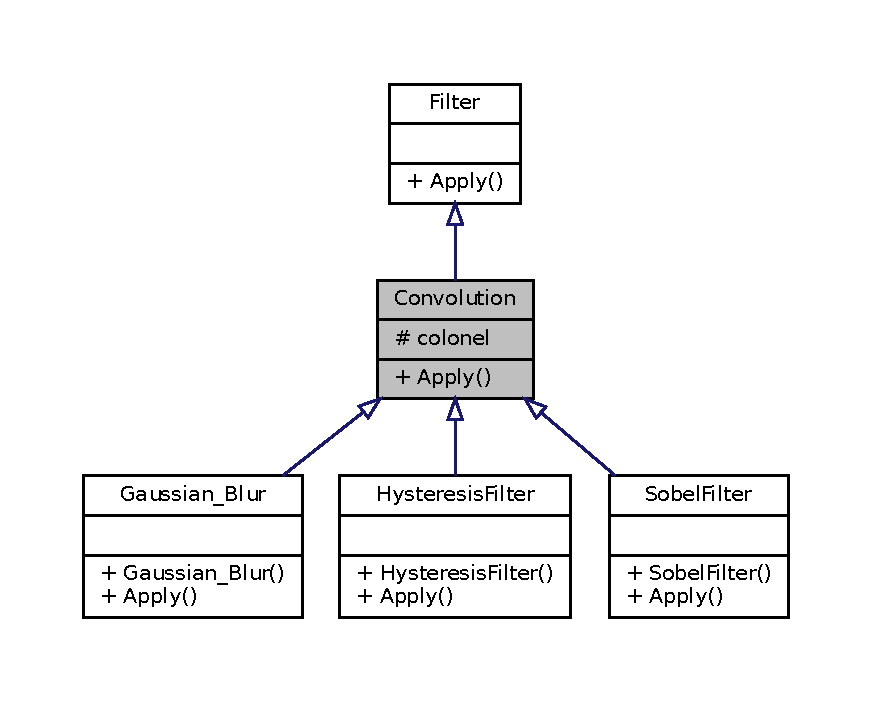
\includegraphics[width=350pt]{classConvolution__inherit__graph}
\end{center}
\end{figure}


Collaboration diagram for Convolution\+:\nopagebreak
\begin{figure}[H]
\begin{center}
\leavevmode
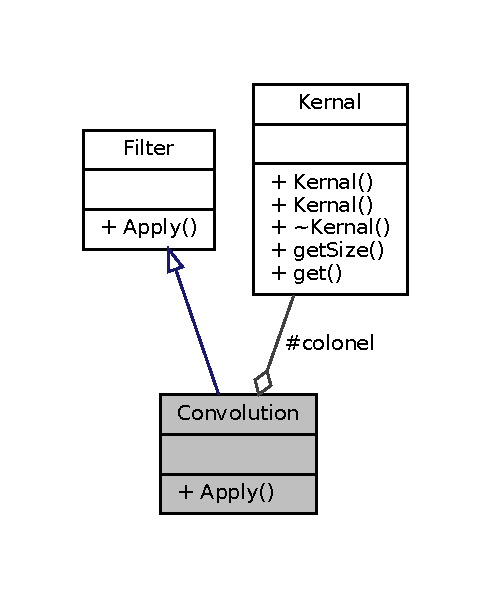
\includegraphics[width=236pt]{classConvolution__coll__graph}
\end{center}
\end{figure}
\doxysubsection*{Public Member Functions}
\begin{DoxyCompactItemize}
\item 
virtual void \mbox{\hyperlink{classConvolution_aaeed86809bdfaa6b5723af9aa06f338c}{Apply}} (std\+::vector$<$ \mbox{\hyperlink{classImage}{Image}} $\ast$ $>$ input, std\+::vector$<$ \mbox{\hyperlink{classImage}{Image}} $\ast$ $>$ output)=0
\begin{DoxyCompactList}\small\item\em apply convolutional filter based on image(s) from input vector, store them in output vector \end{DoxyCompactList}\end{DoxyCompactItemize}
\doxysubsection*{Protected Attributes}
\begin{DoxyCompactItemize}
\item 
\mbox{\Hypertarget{classConvolution_acd84785d396338662bc860668add539f}\label{classConvolution_acd84785d396338662bc860668add539f}} 
\mbox{\hyperlink{classKernal}{Kernal}} {\bfseries colonel}
\end{DoxyCompactItemize}


\doxysubsection{Detailed Description}
The main class for convolutional filters, purely virtual. 



\doxysubsection{Member Function Documentation}
\mbox{\Hypertarget{classConvolution_aaeed86809bdfaa6b5723af9aa06f338c}\label{classConvolution_aaeed86809bdfaa6b5723af9aa06f338c}} 
\index{Convolution@{Convolution}!Apply@{Apply}}
\index{Apply@{Apply}!Convolution@{Convolution}}
\doxysubsubsection{\texorpdfstring{Apply()}{Apply()}}
{\footnotesize\ttfamily virtual void Convolution\+::\+Apply (\begin{DoxyParamCaption}\item[{std\+::vector$<$ \mbox{\hyperlink{classImage}{Image}} $\ast$ $>$}]{input,  }\item[{std\+::vector$<$ \mbox{\hyperlink{classImage}{Image}} $\ast$ $>$}]{output }\end{DoxyParamCaption})\hspace{0.3cm}{\ttfamily [pure virtual]}}



apply convolutional filter based on image(s) from input vector, store them in output vector 

\begin{DoxyReturn}{Returns}
none 
\end{DoxyReturn}


Implements \mbox{\hyperlink{classFilter_a7431e1f16621d96f8a63b37b6907bb04}{Filter}}.



Implemented in \mbox{\hyperlink{classGaussian__Blur_a61c8aabccb7086cd881a222edd1bcfcc}{Gaussian\+\_\+\+Blur}}, \mbox{\hyperlink{classHysteresisFilter_a97979ee97f1105b4b2092ae0e454ca21}{Hysteresis\+Filter}}, and \mbox{\hyperlink{classSobelFilter_a8cafdb5060028072077d4303840962ca}{Sobel\+Filter}}.



The documentation for this class was generated from the following file\+:\begin{DoxyCompactItemize}
\item 
/home/ivers743/3081\+\_\+f21/repo-\/team-\/22/src/img\+\_\+proc\+\_\+src/\mbox{\hyperlink{convolution_8h}{convolution.\+h}}\end{DoxyCompactItemize}

\hypertarget{classDoubleThresholdFilter}{}\section{Double\+Threshold\+Filter Class Reference}
\label{classDoubleThresholdFilter}\index{Double\+Threshold\+Filter@{Double\+Threshold\+Filter}}


The main class of \hyperlink{classDoubleThresholdFilter}{Double\+Threshold\+Filter}.  




{\ttfamily \#include $<$doublethreshold.\+h$>$}



Inheritance diagram for Double\+Threshold\+Filter\+:
\nopagebreak
\begin{figure}[H]
\begin{center}
\leavevmode
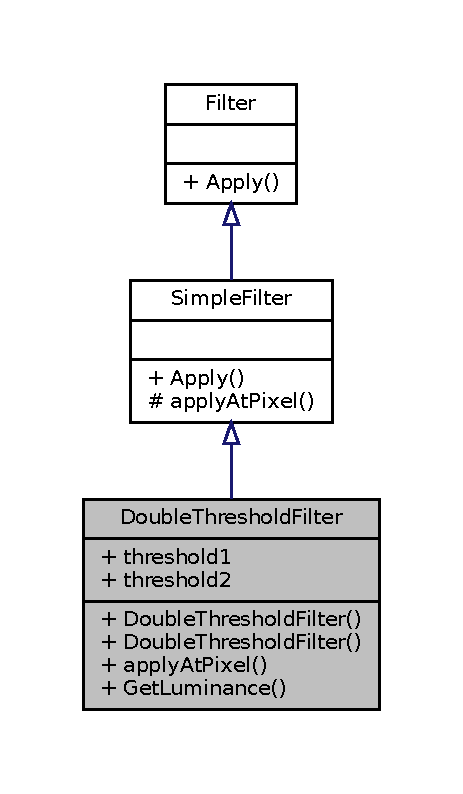
\includegraphics[width=222pt]{classDoubleThresholdFilter__inherit__graph}
\end{center}
\end{figure}


Collaboration diagram for Double\+Threshold\+Filter\+:
\nopagebreak
\begin{figure}[H]
\begin{center}
\leavevmode
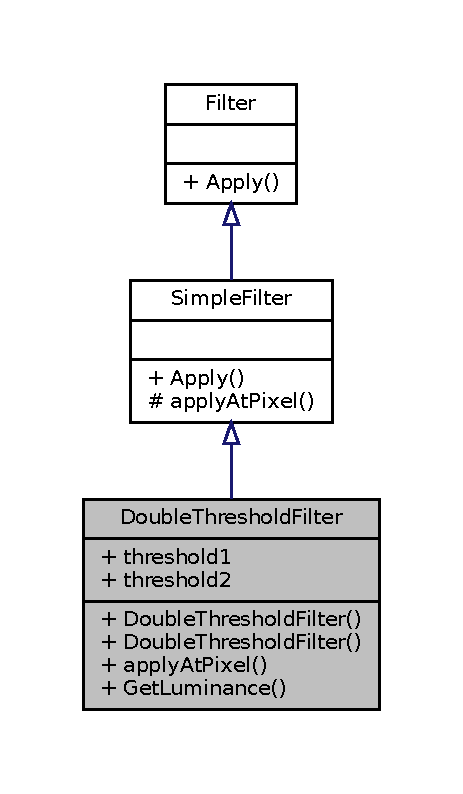
\includegraphics[width=222pt]{classDoubleThresholdFilter__coll__graph}
\end{center}
\end{figure}
\subsection*{Public Member Functions}
\begin{DoxyCompactItemize}
\item 
\mbox{\Hypertarget{classDoubleThresholdFilter_ae4c841df681b376c611e2bc07a2a0d54}\label{classDoubleThresholdFilter_ae4c841df681b376c611e2bc07a2a0d54}} 
\hyperlink{classDoubleThresholdFilter_ae4c841df681b376c611e2bc07a2a0d54}{Double\+Threshold\+Filter} ()
\begin{DoxyCompactList}\small\item\em Generation of a \hyperlink{classDoubleThresholdFilter}{Double\+Threshold\+Filter} with no parameters. \end{DoxyCompactList}\item 
\mbox{\Hypertarget{classDoubleThresholdFilter_a8c65581e746bc42b627df785de7e4512}\label{classDoubleThresholdFilter_a8c65581e746bc42b627df785de7e4512}} 
\hyperlink{classDoubleThresholdFilter_a8c65581e746bc42b627df785de7e4512}{Double\+Threshold\+Filter} (float t1, float t2)
\begin{DoxyCompactList}\small\item\em Generation of a \hyperlink{classDoubleThresholdFilter}{Double\+Threshold\+Filter} with two parameters, the two thresholds to be used in the image calculation. \end{DoxyCompactList}\item 
\mbox{\Hypertarget{classDoubleThresholdFilter_ab6e5b2d489d32913b8cb1854d4ba6db2}\label{classDoubleThresholdFilter_ab6e5b2d489d32913b8cb1854d4ba6db2}} 
unsigned char $\ast$ \hyperlink{classDoubleThresholdFilter_ab6e5b2d489d32913b8cb1854d4ba6db2}{apply\+At\+Pixel} (unsigned char $\ast$pixel)
\begin{DoxyCompactList}\small\item\em Application of a \hyperlink{classDoubleThresholdFilter}{Double\+Threshold\+Filter} at a specific pixel in the image. \end{DoxyCompactList}\item 
\mbox{\Hypertarget{classDoubleThresholdFilter_a1881b9f96b709926b6e64a6e67eea44a}\label{classDoubleThresholdFilter_a1881b9f96b709926b6e64a6e67eea44a}} 
float \hyperlink{classDoubleThresholdFilter_a1881b9f96b709926b6e64a6e67eea44a}{Get\+Luminance} (float red, float green, float blue)
\begin{DoxyCompactList}\small\item\em Returns the Luminance of a specific pixel with a simple equation in order to determine what threshold it falls in. \end{DoxyCompactList}\end{DoxyCompactItemize}
\subsection*{Public Attributes}
\begin{DoxyCompactItemize}
\item 
\mbox{\Hypertarget{classDoubleThresholdFilter_a7e42f69279e156d747011690456cea20}\label{classDoubleThresholdFilter_a7e42f69279e156d747011690456cea20}} 
float \hyperlink{classDoubleThresholdFilter_a7e42f69279e156d747011690456cea20}{threshold1}
\begin{DoxyCompactList}\small\item\em The two thresholds that define the look of the output image. \end{DoxyCompactList}\item 
\mbox{\Hypertarget{classDoubleThresholdFilter_ae4f4aafd4245d8682c7456f7430e4886}\label{classDoubleThresholdFilter_ae4f4aafd4245d8682c7456f7430e4886}} 
float {\bfseries threshold2}
\end{DoxyCompactItemize}
\subsection*{Additional Inherited Members}


\subsection{Detailed Description}
The main class of \hyperlink{classDoubleThresholdFilter}{Double\+Threshold\+Filter}. 

Derived class of \hyperlink{classSimpleFilter}{Simple\+Filter}, invoked to create and apply a double threshold filter to an \hyperlink{classImage}{Image}. 

The documentation for this class was generated from the following files\+:\begin{DoxyCompactItemize}
\item 
/home/user/repo/\hyperlink{doublethreshold_8h}{doublethreshold.\+h}\item 
/home/user/repo/doublethreshold.\+cc\end{DoxyCompactItemize}

\hypertarget{classFilter}{}\doxysection{Filter Class Reference}
\label{classFilter}\index{Filter@{Filter}}


The main class for filters, purely virtual.  




{\ttfamily \#include $<$filter.\+h$>$}



Inheritance diagram for Filter\+:\nopagebreak
\begin{figure}[H]
\begin{center}
\leavevmode
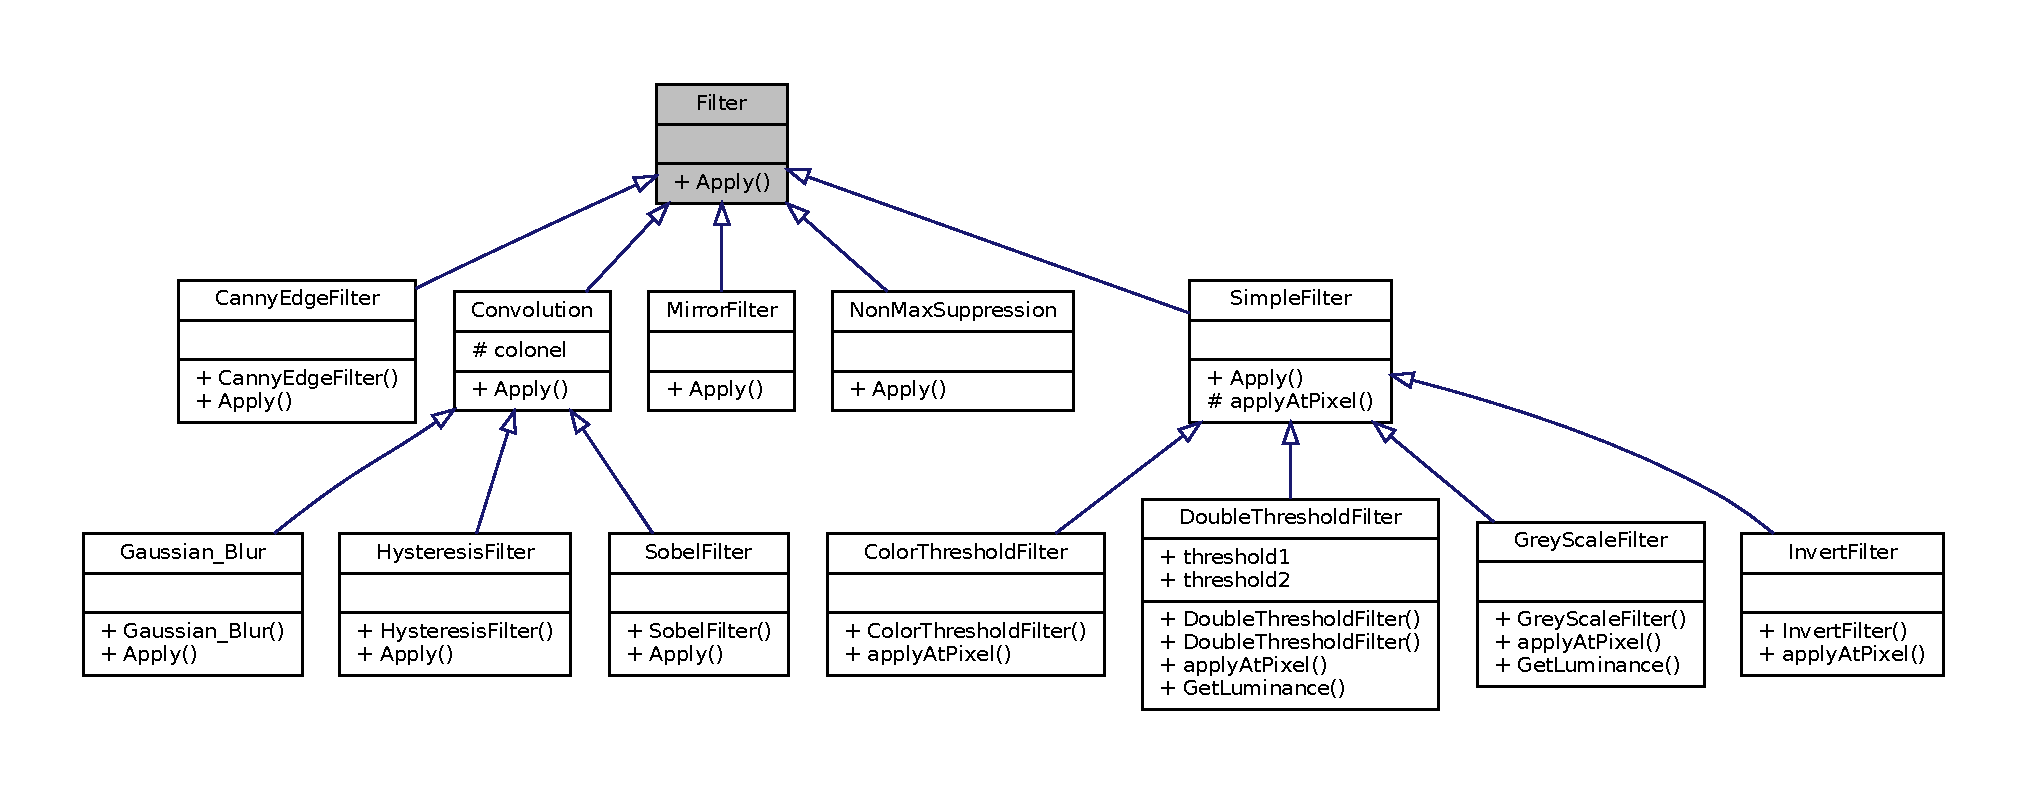
\includegraphics[width=276pt]{classFilter__inherit__graph}
\end{center}
\end{figure}


Collaboration diagram for Filter\+:\nopagebreak
\begin{figure}[H]
\begin{center}
\leavevmode
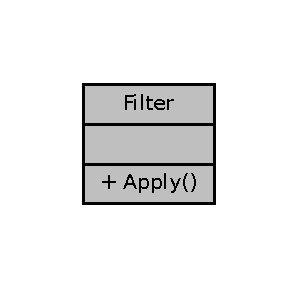
\includegraphics[width=143pt]{classFilter__coll__graph}
\end{center}
\end{figure}
\doxysubsection*{Public Member Functions}
\begin{DoxyCompactItemize}
\item 
virtual void \mbox{\hyperlink{classFilter_a7431e1f16621d96f8a63b37b6907bb04}{Apply}} (std\+::vector$<$ \mbox{\hyperlink{classImage}{Image}} $\ast$ $>$ original, std\+::vector$<$ \mbox{\hyperlink{classImage}{Image}} $\ast$ $>$ filtered)=0
\begin{DoxyCompactList}\small\item\em apply convolutional filter based on image(s) from input vector, store them in output vector \end{DoxyCompactList}\end{DoxyCompactItemize}


\doxysubsection{Detailed Description}
The main class for filters, purely virtual. 



\doxysubsection{Member Function Documentation}
\mbox{\Hypertarget{classFilter_a7431e1f16621d96f8a63b37b6907bb04}\label{classFilter_a7431e1f16621d96f8a63b37b6907bb04}} 
\index{Filter@{Filter}!Apply@{Apply}}
\index{Apply@{Apply}!Filter@{Filter}}
\doxysubsubsection{\texorpdfstring{Apply()}{Apply()}}
{\footnotesize\ttfamily virtual void Filter\+::\+Apply (\begin{DoxyParamCaption}\item[{std\+::vector$<$ \mbox{\hyperlink{classImage}{Image}} $\ast$ $>$}]{original,  }\item[{std\+::vector$<$ \mbox{\hyperlink{classImage}{Image}} $\ast$ $>$}]{filtered }\end{DoxyParamCaption})\hspace{0.3cm}{\ttfamily [pure virtual]}}



apply convolutional filter based on image(s) from input vector, store them in output vector 

\begin{DoxyReturn}{Returns}
none 
\end{DoxyReturn}


Implemented in \mbox{\hyperlink{classSimpleFilter_a66dc06c85d8a38487e3dddc3e1731f37}{Simple\+Filter}}, and \mbox{\hyperlink{classConvolution_aaeed86809bdfaa6b5723af9aa06f338c}{Convolution}}.



The documentation for this class was generated from the following file\+:\begin{DoxyCompactItemize}
\item 
/home/ivers743/3081\+\_\+f21/repo-\/team-\/22/\mbox{\hyperlink{filter_8h}{filter.\+h}}\end{DoxyCompactItemize}

\hypertarget{classGaussian__Blur}{}\doxysection{Gaussian\+\_\+\+Blur Class Reference}
\label{classGaussian__Blur}\index{Gaussian\_Blur@{Gaussian\_Blur}}


Gaussian Blur class, allows for the creation of gaussian blur filters.  




{\ttfamily \#include $<$gaussian\+\_\+blur.\+h$>$}



Inheritance diagram for Gaussian\+\_\+\+Blur\+:\nopagebreak
\begin{figure}[H]
\begin{center}
\leavevmode
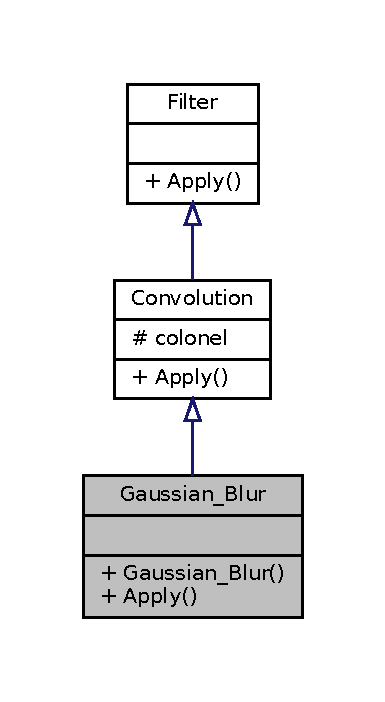
\includegraphics[width=185pt]{classGaussian__Blur__inherit__graph}
\end{center}
\end{figure}


Collaboration diagram for Gaussian\+\_\+\+Blur\+:\nopagebreak
\begin{figure}[H]
\begin{center}
\leavevmode
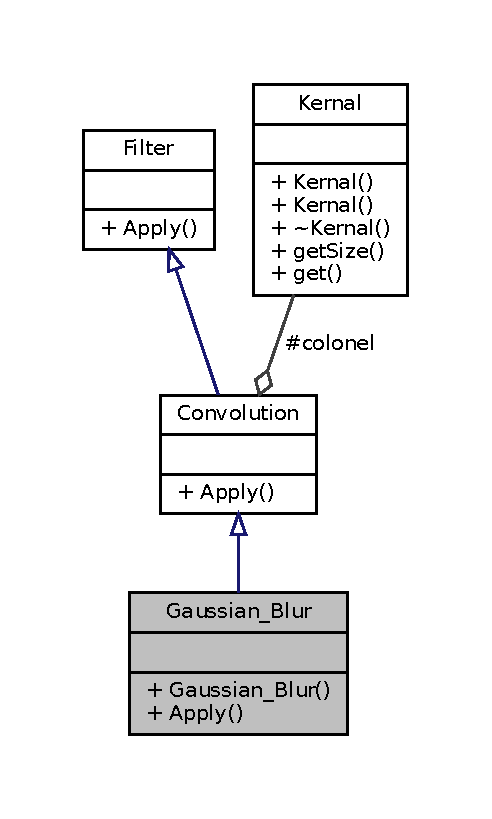
\includegraphics[width=236pt]{classGaussian__Blur__coll__graph}
\end{center}
\end{figure}
\doxysubsection*{Public Member Functions}
\begin{DoxyCompactItemize}
\item 
\mbox{\hyperlink{classGaussian__Blur_a6578511e43e84f3c7bc9356324df223e}{Gaussian\+\_\+\+Blur}} ()
\begin{DoxyCompactList}\small\item\em constructor, sets colonel to the gaussian identity matrix \end{DoxyCompactList}\item 
void \mbox{\hyperlink{classGaussian__Blur_a61c8aabccb7086cd881a222edd1bcfcc}{Apply}} (std\+::vector$<$ \mbox{\hyperlink{classImage}{Image}} $\ast$ $>$ original, std\+::vector$<$ \mbox{\hyperlink{classImage}{Image}} $\ast$ $>$ filtered)
\begin{DoxyCompactList}\small\item\em method to apply gaussian blur to an image \end{DoxyCompactList}\end{DoxyCompactItemize}
\doxysubsection*{Additional Inherited Members}


\doxysubsection{Detailed Description}
Gaussian Blur class, allows for the creation of gaussian blur filters. 



\doxysubsection{Constructor \& Destructor Documentation}
\mbox{\Hypertarget{classGaussian__Blur_a6578511e43e84f3c7bc9356324df223e}\label{classGaussian__Blur_a6578511e43e84f3c7bc9356324df223e}} 
\index{Gaussian\_Blur@{Gaussian\_Blur}!Gaussian\_Blur@{Gaussian\_Blur}}
\index{Gaussian\_Blur@{Gaussian\_Blur}!Gaussian\_Blur@{Gaussian\_Blur}}
\doxysubsubsection{\texorpdfstring{Gaussian\_Blur()}{Gaussian\_Blur()}}
{\footnotesize\ttfamily Gaussian\+\_\+\+Blur\+::\+Gaussian\+\_\+\+Blur (\begin{DoxyParamCaption}{ }\end{DoxyParamCaption})}



constructor, sets colonel to the gaussian identity matrix 



\doxysubsection{Member Function Documentation}
\mbox{\Hypertarget{classGaussian__Blur_a61c8aabccb7086cd881a222edd1bcfcc}\label{classGaussian__Blur_a61c8aabccb7086cd881a222edd1bcfcc}} 
\index{Gaussian\_Blur@{Gaussian\_Blur}!Apply@{Apply}}
\index{Apply@{Apply}!Gaussian\_Blur@{Gaussian\_Blur}}
\doxysubsubsection{\texorpdfstring{Apply()}{Apply()}}
{\footnotesize\ttfamily void Gaussian\+\_\+\+Blur\+::\+Apply (\begin{DoxyParamCaption}\item[{std\+::vector$<$ \mbox{\hyperlink{classImage}{Image}} $\ast$ $>$}]{original,  }\item[{std\+::vector$<$ \mbox{\hyperlink{classImage}{Image}} $\ast$ $>$}]{filtered }\end{DoxyParamCaption})\hspace{0.3cm}{\ttfamily [virtual]}}



method to apply gaussian blur to an image 



Implements \mbox{\hyperlink{classConvolution_aaeed86809bdfaa6b5723af9aa06f338c}{Convolution}}.



The documentation for this class was generated from the following files\+:\begin{DoxyCompactItemize}
\item 
/home/ivers743/3081\+\_\+f21/repo-\/team-\/22/src/img\+\_\+proc\+\_\+src/\mbox{\hyperlink{gaussian__blur_8h}{gaussian\+\_\+blur.\+h}}\item 
/home/ivers743/3081\+\_\+f21/repo-\/team-\/22/src/img\+\_\+proc\+\_\+src/gaussian\+\_\+blur.\+cc\end{DoxyCompactItemize}

\hypertarget{classGreyScaleFilter}{}\doxysection{Grey\+Scale\+Filter Class Reference}
\label{classGreyScaleFilter}\index{GreyScaleFilter@{GreyScaleFilter}}


greyscale filter class, applies the greyscale filter to an image  




{\ttfamily \#include $<$greyscale\+\_\+filter.\+h$>$}



Inheritance diagram for Grey\+Scale\+Filter\+:\nopagebreak
\begin{figure}[H]
\begin{center}
\leavevmode
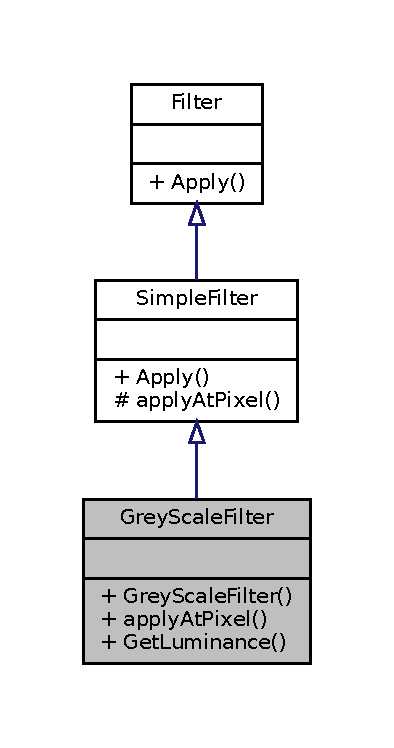
\includegraphics[width=189pt]{classGreyScaleFilter__inherit__graph}
\end{center}
\end{figure}


Collaboration diagram for Grey\+Scale\+Filter\+:\nopagebreak
\begin{figure}[H]
\begin{center}
\leavevmode
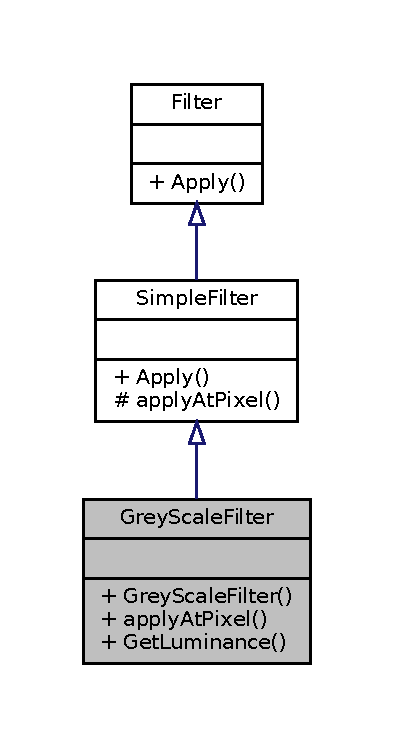
\includegraphics[width=189pt]{classGreyScaleFilter__coll__graph}
\end{center}
\end{figure}
\doxysubsection*{Public Member Functions}
\begin{DoxyCompactItemize}
\item 
\mbox{\hyperlink{classGreyScaleFilter_a39c97682b954a5c00135eb4c13bddd47}{Grey\+Scale\+Filter}} ()
\begin{DoxyCompactList}\small\item\em constructor for creating a \mbox{\hyperlink{classGreyScaleFilter}{Grey\+Scale\+Filter}} \end{DoxyCompactList}\item 
unsigned char $\ast$ \mbox{\hyperlink{classGreyScaleFilter_afac3eb54599341d326d9df20de67f851}{apply\+At\+Pixel}} (unsigned char $\ast$pixel)
\begin{DoxyCompactList}\small\item\em apply convolutional filter based on image(s) from input vector, store them in output vector \end{DoxyCompactList}\item 
float \mbox{\hyperlink{classGreyScaleFilter_a89a03b17fa1ee8c556eeb173b11bf4e4}{Get\+Luminance}} (float red, float green, float blue)
\begin{DoxyCompactList}\small\item\em get the luminance of a pixel \end{DoxyCompactList}\end{DoxyCompactItemize}
\doxysubsection*{Additional Inherited Members}


\doxysubsection{Detailed Description}
greyscale filter class, applies the greyscale filter to an image 



\doxysubsection{Constructor \& Destructor Documentation}
\mbox{\Hypertarget{classGreyScaleFilter_a39c97682b954a5c00135eb4c13bddd47}\label{classGreyScaleFilter_a39c97682b954a5c00135eb4c13bddd47}} 
\index{GreyScaleFilter@{GreyScaleFilter}!GreyScaleFilter@{GreyScaleFilter}}
\index{GreyScaleFilter@{GreyScaleFilter}!GreyScaleFilter@{GreyScaleFilter}}
\doxysubsubsection{\texorpdfstring{GreyScaleFilter()}{GreyScaleFilter()}}
{\footnotesize\ttfamily Grey\+Scale\+Filter\+::\+Grey\+Scale\+Filter (\begin{DoxyParamCaption}{ }\end{DoxyParamCaption})}



constructor for creating a \mbox{\hyperlink{classGreyScaleFilter}{Grey\+Scale\+Filter}} 

\begin{DoxyReturn}{Returns}
a \mbox{\hyperlink{classGreyScaleFilter}{Grey\+Scale\+Filter}} object 
\end{DoxyReturn}


\doxysubsection{Member Function Documentation}
\mbox{\Hypertarget{classGreyScaleFilter_afac3eb54599341d326d9df20de67f851}\label{classGreyScaleFilter_afac3eb54599341d326d9df20de67f851}} 
\index{GreyScaleFilter@{GreyScaleFilter}!applyAtPixel@{applyAtPixel}}
\index{applyAtPixel@{applyAtPixel}!GreyScaleFilter@{GreyScaleFilter}}
\doxysubsubsection{\texorpdfstring{applyAtPixel()}{applyAtPixel()}}
{\footnotesize\ttfamily unsigned char $\ast$ Grey\+Scale\+Filter\+::apply\+At\+Pixel (\begin{DoxyParamCaption}\item[{unsigned char $\ast$}]{pixel }\end{DoxyParamCaption})\hspace{0.3cm}{\ttfamily [virtual]}}



apply convolutional filter based on image(s) from input vector, store them in output vector 

\begin{DoxyReturn}{Returns}
a length 4 unsigned char array of values 
\end{DoxyReturn}


Implements \mbox{\hyperlink{classSimpleFilter_a24100e6c29c4bf3bddf2763c22622d75}{Simple\+Filter}}.

\mbox{\Hypertarget{classGreyScaleFilter_a89a03b17fa1ee8c556eeb173b11bf4e4}\label{classGreyScaleFilter_a89a03b17fa1ee8c556eeb173b11bf4e4}} 
\index{GreyScaleFilter@{GreyScaleFilter}!GetLuminance@{GetLuminance}}
\index{GetLuminance@{GetLuminance}!GreyScaleFilter@{GreyScaleFilter}}
\doxysubsubsection{\texorpdfstring{GetLuminance()}{GetLuminance()}}
{\footnotesize\ttfamily float Grey\+Scale\+Filter\+::\+Get\+Luminance (\begin{DoxyParamCaption}\item[{float}]{red,  }\item[{float}]{green,  }\item[{float}]{blue }\end{DoxyParamCaption})}



get the luminance of a pixel 

\begin{DoxyReturn}{Returns}
a float representing the luminance of an image 
\end{DoxyReturn}


The documentation for this class was generated from the following files\+:\begin{DoxyCompactItemize}
\item 
/home/ivers743/3081\+\_\+f21/repo-\/team-\/22/src/img\+\_\+proc\+\_\+src/\mbox{\hyperlink{greyscale__filter_8h}{greyscale\+\_\+filter.\+h}}\item 
/home/ivers743/3081\+\_\+f21/repo-\/team-\/22/src/img\+\_\+proc\+\_\+src/greyscale\+\_\+filter.\+cc\end{DoxyCompactItemize}

\hypertarget{classHysteresisFilter}{}\doxysection{Hysteresis\+Filter Class Reference}
\label{classHysteresisFilter}\index{HysteresisFilter@{HysteresisFilter}}


Hysteresis \mbox{\hyperlink{classFilter}{Filter}} class, allows for the creation of hysteresis filters.  




{\ttfamily \#include $<$hysteresis\+\_\+filter.\+h$>$}



Inheritance diagram for Hysteresis\+Filter\+:\nopagebreak
\begin{figure}[H]
\begin{center}
\leavevmode
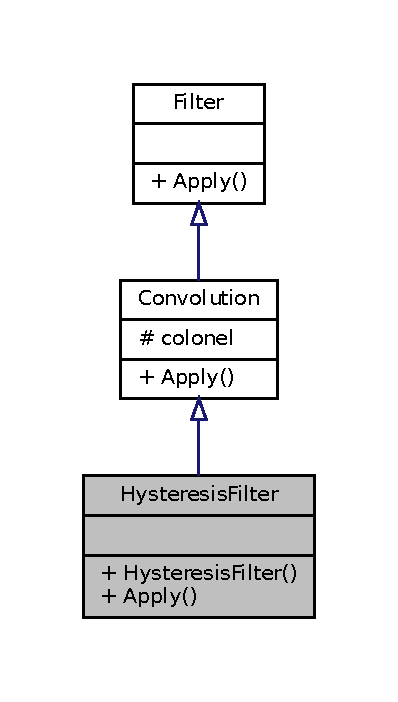
\includegraphics[width=191pt]{classHysteresisFilter__inherit__graph}
\end{center}
\end{figure}


Collaboration diagram for Hysteresis\+Filter\+:\nopagebreak
\begin{figure}[H]
\begin{center}
\leavevmode
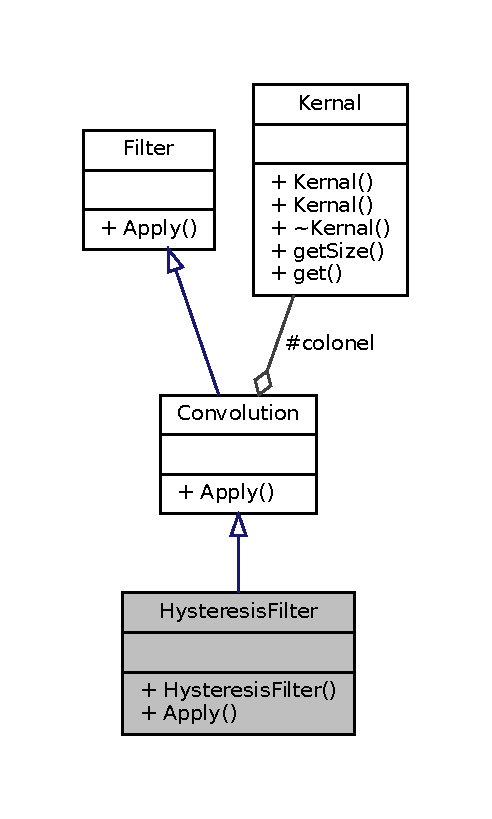
\includegraphics[width=236pt]{classHysteresisFilter__coll__graph}
\end{center}
\end{figure}
\doxysubsection*{Public Member Functions}
\begin{DoxyCompactItemize}
\item 
\mbox{\hyperlink{classHysteresisFilter_afe7c944e6233cc9c698868d683f5083d}{Hysteresis\+Filter}} ()
\begin{DoxyCompactList}\small\item\em constructor, sets colonel to a 3x3 \end{DoxyCompactList}\item 
void \mbox{\hyperlink{classHysteresisFilter_a97979ee97f1105b4b2092ae0e454ca21}{Apply}} (std\+::vector$<$ \mbox{\hyperlink{classImage}{Image}} $\ast$ $>$ original, std\+::vector$<$ \mbox{\hyperlink{classImage}{Image}} $\ast$ $>$ filtered)
\begin{DoxyCompactList}\small\item\em method to apply hysteresis to an image \end{DoxyCompactList}\end{DoxyCompactItemize}
\doxysubsection*{Additional Inherited Members}


\doxysubsection{Detailed Description}
Hysteresis \mbox{\hyperlink{classFilter}{Filter}} class, allows for the creation of hysteresis filters. 



\doxysubsection{Constructor \& Destructor Documentation}
\mbox{\Hypertarget{classHysteresisFilter_afe7c944e6233cc9c698868d683f5083d}\label{classHysteresisFilter_afe7c944e6233cc9c698868d683f5083d}} 
\index{HysteresisFilter@{HysteresisFilter}!HysteresisFilter@{HysteresisFilter}}
\index{HysteresisFilter@{HysteresisFilter}!HysteresisFilter@{HysteresisFilter}}
\doxysubsubsection{\texorpdfstring{HysteresisFilter()}{HysteresisFilter()}}
{\footnotesize\ttfamily Hysteresis\+Filter\+::\+Hysteresis\+Filter (\begin{DoxyParamCaption}{ }\end{DoxyParamCaption})}



constructor, sets colonel to a 3x3 



\doxysubsection{Member Function Documentation}
\mbox{\Hypertarget{classHysteresisFilter_a97979ee97f1105b4b2092ae0e454ca21}\label{classHysteresisFilter_a97979ee97f1105b4b2092ae0e454ca21}} 
\index{HysteresisFilter@{HysteresisFilter}!Apply@{Apply}}
\index{Apply@{Apply}!HysteresisFilter@{HysteresisFilter}}
\doxysubsubsection{\texorpdfstring{Apply()}{Apply()}}
{\footnotesize\ttfamily void Hysteresis\+Filter\+::\+Apply (\begin{DoxyParamCaption}\item[{std\+::vector$<$ \mbox{\hyperlink{classImage}{Image}} $\ast$ $>$}]{original,  }\item[{std\+::vector$<$ \mbox{\hyperlink{classImage}{Image}} $\ast$ $>$}]{filtered }\end{DoxyParamCaption})\hspace{0.3cm}{\ttfamily [virtual]}}



method to apply hysteresis to an image 



Implements \mbox{\hyperlink{classConvolution_aaeed86809bdfaa6b5723af9aa06f338c}{Convolution}}.



The documentation for this class was generated from the following files\+:\begin{DoxyCompactItemize}
\item 
/home/ivers743/3081\+\_\+f21/repo-\/team-\/22/src/img\+\_\+proc\+\_\+src/\mbox{\hyperlink{hysteresis__filter_8h}{hysteresis\+\_\+filter.\+h}}\item 
/home/ivers743/3081\+\_\+f21/repo-\/team-\/22/src/img\+\_\+proc\+\_\+src/hysteresis\+\_\+filter.\+cc\end{DoxyCompactItemize}

\hypertarget{classImage}{}\doxysection{Image Class Reference}
\label{classImage}\index{Image@{Image}}


The main class for images, allows for copying, saving, and getting/setting pixels.  




{\ttfamily \#include $<$image.\+h$>$}



Collaboration diagram for Image\+:\nopagebreak
\begin{figure}[H]
\begin{center}
\leavevmode
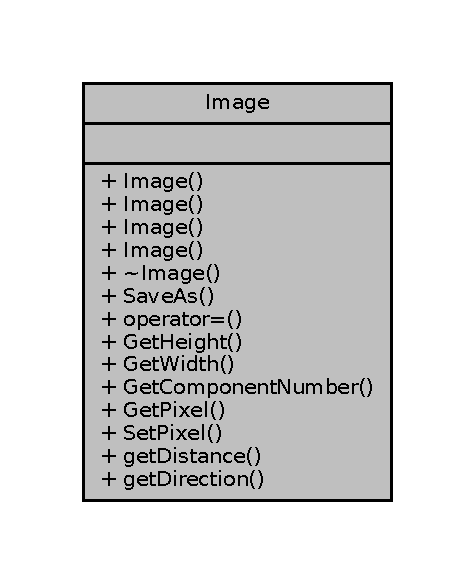
\includegraphics[width=228pt]{classImage__coll__graph}
\end{center}
\end{figure}
\doxysubsection*{Public Member Functions}
\begin{DoxyCompactItemize}
\item 
\mbox{\hyperlink{classImage_a58edd1c45b4faeb5f789b0d036d02313}{Image}} ()
\begin{DoxyCompactList}\small\item\em default constructor for creating an image; \end{DoxyCompactList}\item 
\mbox{\hyperlink{classImage_afb0339b802ed560e69eb07358d30198f}{Image}} (int width, int height)
\begin{DoxyCompactList}\small\item\em a constructor for creating an image; \end{DoxyCompactList}\item 
\mbox{\hyperlink{classImage_a5ab2d611b6c128521a51380c25843f49}{Image}} (std\+::string fname)
\begin{DoxyCompactList}\small\item\em a constructor for creating an image; \end{DoxyCompactList}\item 
\mbox{\hyperlink{classImage_a34410a36b132ab597a8878d45facc89a}{Image}} (const \mbox{\hyperlink{classImage}{Image}} \&image)
\begin{DoxyCompactList}\small\item\em a copy constructor for creating an image; \end{DoxyCompactList}\item 
\mbox{\hyperlink{classImage_a0294f63700543e11c0f0da85601c7ae5}{$\sim$\+Image}} ()
\begin{DoxyCompactList}\small\item\em destructor for an image; \end{DoxyCompactList}\item 
void \mbox{\hyperlink{classImage_a7884b109eec6cdc52295011f4e0552fd}{Save\+As}} (std\+::string fname)
\begin{DoxyCompactList}\small\item\em Saves the image to the file fname;. \end{DoxyCompactList}\item 
void \mbox{\hyperlink{classImage_ad87aee5af20779f84891b08b23319ce2}{operator=}} (\mbox{\hyperlink{classImage}{Image}} image)
\begin{DoxyCompactList}\small\item\em equals operator for setting an image; \end{DoxyCompactList}\item 
int \mbox{\hyperlink{classImage_a4d6de643ee334ff52c85da9a62d9297d}{Get\+Height}} ()
\begin{DoxyCompactList}\small\item\em getter for the width of an image; \end{DoxyCompactList}\item 
int \mbox{\hyperlink{classImage_a4ab80d76fd124fd9de9b4fca8ae16186}{Get\+Width}} ()
\begin{DoxyCompactList}\small\item\em getter for the height of the image; \end{DoxyCompactList}\item 
int \mbox{\hyperlink{classImage_a34d2edb4e483b17babd5f0026f7c2ab0}{Get\+Component\+Number}} ()
\begin{DoxyCompactList}\small\item\em a function for getting the number of components of an image; \end{DoxyCompactList}\item 
unsigned char $\ast$ \mbox{\hyperlink{classImage_aa0b312879805efe9b0bf50929383026d}{Get\+Pixel}} (int x, int y)
\begin{DoxyCompactList}\small\item\em a getter for the pixel located at (x,y); \end{DoxyCompactList}\item 
void \mbox{\hyperlink{classImage_a70147670b58d1b095e5c38b1f8bfb2db}{Set\+Pixel}} (int x, int y, unsigned char $\ast$colors)
\begin{DoxyCompactList}\small\item\em setter for pixel at(x,y) to be set with the unsigned char array colors; \end{DoxyCompactList}\item 
\mbox{\Hypertarget{classImage_a83ff2d122d7ed917ba8ea475ed35f199}\label{classImage_a83ff2d122d7ed917ba8ea475ed35f199}} 
float {\bfseries get\+Distance} (int x, int y)
\item 
\mbox{\Hypertarget{classImage_aad9e00ee8b282ad7f3d4b40c04661594}\label{classImage_aad9e00ee8b282ad7f3d4b40c04661594}} 
std\+::vector$<$ float $>$ {\bfseries get\+Direction} (int x, int y)
\end{DoxyCompactItemize}


\doxysubsection{Detailed Description}
The main class for images, allows for copying, saving, and getting/setting pixels. 



\doxysubsection{Constructor \& Destructor Documentation}
\mbox{\Hypertarget{classImage_a58edd1c45b4faeb5f789b0d036d02313}\label{classImage_a58edd1c45b4faeb5f789b0d036d02313}} 
\index{Image@{Image}!Image@{Image}}
\index{Image@{Image}!Image@{Image}}
\doxysubsubsection{\texorpdfstring{Image()}{Image()}\hspace{0.1cm}{\footnotesize\ttfamily [1/4]}}
{\footnotesize\ttfamily Image\+::\+Image (\begin{DoxyParamCaption}{ }\end{DoxyParamCaption})}



default constructor for creating an image; 

\begin{DoxyReturn}{Returns}
an \mbox{\hyperlink{classImage}{Image}} with width 0 and height 0; 
\end{DoxyReturn}
\mbox{\Hypertarget{classImage_afb0339b802ed560e69eb07358d30198f}\label{classImage_afb0339b802ed560e69eb07358d30198f}} 
\index{Image@{Image}!Image@{Image}}
\index{Image@{Image}!Image@{Image}}
\doxysubsubsection{\texorpdfstring{Image()}{Image()}\hspace{0.1cm}{\footnotesize\ttfamily [2/4]}}
{\footnotesize\ttfamily Image\+::\+Image (\begin{DoxyParamCaption}\item[{int}]{width,  }\item[{int}]{height }\end{DoxyParamCaption})}



a constructor for creating an image; 

\begin{DoxyReturn}{Returns}
an \mbox{\hyperlink{classImage}{Image}} with a certain width and height; 
\end{DoxyReturn}
\mbox{\Hypertarget{classImage_a5ab2d611b6c128521a51380c25843f49}\label{classImage_a5ab2d611b6c128521a51380c25843f49}} 
\index{Image@{Image}!Image@{Image}}
\index{Image@{Image}!Image@{Image}}
\doxysubsubsection{\texorpdfstring{Image()}{Image()}\hspace{0.1cm}{\footnotesize\ttfamily [3/4]}}
{\footnotesize\ttfamily Image\+::\+Image (\begin{DoxyParamCaption}\item[{std\+::string}]{fname }\end{DoxyParamCaption})}



a constructor for creating an image; 

\begin{DoxyReturn}{Returns}
an \mbox{\hyperlink{classImage}{Image}} read in from a file fname; 
\end{DoxyReturn}
\mbox{\Hypertarget{classImage_a34410a36b132ab597a8878d45facc89a}\label{classImage_a34410a36b132ab597a8878d45facc89a}} 
\index{Image@{Image}!Image@{Image}}
\index{Image@{Image}!Image@{Image}}
\doxysubsubsection{\texorpdfstring{Image()}{Image()}\hspace{0.1cm}{\footnotesize\ttfamily [4/4]}}
{\footnotesize\ttfamily Image\+::\+Image (\begin{DoxyParamCaption}\item[{const \mbox{\hyperlink{classImage}{Image}} \&}]{image }\end{DoxyParamCaption})}



a copy constructor for creating an image; 

\begin{DoxyReturn}{Returns}
an \mbox{\hyperlink{classImage}{Image}} identical to the one passed in; 
\end{DoxyReturn}
\mbox{\Hypertarget{classImage_a0294f63700543e11c0f0da85601c7ae5}\label{classImage_a0294f63700543e11c0f0da85601c7ae5}} 
\index{Image@{Image}!````~Image@{$\sim$Image}}
\index{````~Image@{$\sim$Image}!Image@{Image}}
\doxysubsubsection{\texorpdfstring{$\sim$Image()}{~Image()}}
{\footnotesize\ttfamily Image\+::$\sim$\+Image (\begin{DoxyParamCaption}{ }\end{DoxyParamCaption})}



destructor for an image; 

\begin{DoxyReturn}{Returns}
none; 
\end{DoxyReturn}


\doxysubsection{Member Function Documentation}
\mbox{\Hypertarget{classImage_a34d2edb4e483b17babd5f0026f7c2ab0}\label{classImage_a34d2edb4e483b17babd5f0026f7c2ab0}} 
\index{Image@{Image}!GetComponentNumber@{GetComponentNumber}}
\index{GetComponentNumber@{GetComponentNumber}!Image@{Image}}
\doxysubsubsection{\texorpdfstring{GetComponentNumber()}{GetComponentNumber()}}
{\footnotesize\ttfamily int Image\+::\+Get\+Component\+Number (\begin{DoxyParamCaption}{ }\end{DoxyParamCaption})}



a function for getting the number of components of an image; 

\begin{DoxyReturn}{Returns}
the number of components as an int; 
\end{DoxyReturn}
\mbox{\Hypertarget{classImage_a4d6de643ee334ff52c85da9a62d9297d}\label{classImage_a4d6de643ee334ff52c85da9a62d9297d}} 
\index{Image@{Image}!GetHeight@{GetHeight}}
\index{GetHeight@{GetHeight}!Image@{Image}}
\doxysubsubsection{\texorpdfstring{GetHeight()}{GetHeight()}}
{\footnotesize\ttfamily int Image\+::\+Get\+Height (\begin{DoxyParamCaption}{ }\end{DoxyParamCaption})}



getter for the width of an image; 

\begin{DoxyReturn}{Returns}
the width of an image as an int; 
\end{DoxyReturn}
\mbox{\Hypertarget{classImage_aa0b312879805efe9b0bf50929383026d}\label{classImage_aa0b312879805efe9b0bf50929383026d}} 
\index{Image@{Image}!GetPixel@{GetPixel}}
\index{GetPixel@{GetPixel}!Image@{Image}}
\doxysubsubsection{\texorpdfstring{GetPixel()}{GetPixel()}}
{\footnotesize\ttfamily unsigned char $\ast$ Image\+::\+Get\+Pixel (\begin{DoxyParamCaption}\item[{int}]{x,  }\item[{int}]{y }\end{DoxyParamCaption})}



a getter for the pixel located at (x,y); 

\begin{DoxyReturn}{Returns}
the length 4 unsigned char array of that pixel; 
\end{DoxyReturn}
\mbox{\Hypertarget{classImage_a4ab80d76fd124fd9de9b4fca8ae16186}\label{classImage_a4ab80d76fd124fd9de9b4fca8ae16186}} 
\index{Image@{Image}!GetWidth@{GetWidth}}
\index{GetWidth@{GetWidth}!Image@{Image}}
\doxysubsubsection{\texorpdfstring{GetWidth()}{GetWidth()}}
{\footnotesize\ttfamily int Image\+::\+Get\+Width (\begin{DoxyParamCaption}{ }\end{DoxyParamCaption})}



getter for the height of the image; 

\begin{DoxyReturn}{Returns}
the height of an image as an int; 
\end{DoxyReturn}
\mbox{\Hypertarget{classImage_ad87aee5af20779f84891b08b23319ce2}\label{classImage_ad87aee5af20779f84891b08b23319ce2}} 
\index{Image@{Image}!operator=@{operator=}}
\index{operator=@{operator=}!Image@{Image}}
\doxysubsubsection{\texorpdfstring{operator=()}{operator=()}}
{\footnotesize\ttfamily void Image\+::operator= (\begin{DoxyParamCaption}\item[{\mbox{\hyperlink{classImage}{Image}}}]{image }\end{DoxyParamCaption})}



equals operator for setting an image; 

\begin{DoxyReturn}{Returns}
none; 
\end{DoxyReturn}
\mbox{\Hypertarget{classImage_a7884b109eec6cdc52295011f4e0552fd}\label{classImage_a7884b109eec6cdc52295011f4e0552fd}} 
\index{Image@{Image}!SaveAs@{SaveAs}}
\index{SaveAs@{SaveAs}!Image@{Image}}
\doxysubsubsection{\texorpdfstring{SaveAs()}{SaveAs()}}
{\footnotesize\ttfamily void Image\+::\+Save\+As (\begin{DoxyParamCaption}\item[{std\+::string}]{fname }\end{DoxyParamCaption})}



Saves the image to the file fname;. 

\begin{DoxyReturn}{Returns}
none; 
\end{DoxyReturn}
\mbox{\Hypertarget{classImage_a70147670b58d1b095e5c38b1f8bfb2db}\label{classImage_a70147670b58d1b095e5c38b1f8bfb2db}} 
\index{Image@{Image}!SetPixel@{SetPixel}}
\index{SetPixel@{SetPixel}!Image@{Image}}
\doxysubsubsection{\texorpdfstring{SetPixel()}{SetPixel()}}
{\footnotesize\ttfamily void Image\+::\+Set\+Pixel (\begin{DoxyParamCaption}\item[{int}]{x,  }\item[{int}]{y,  }\item[{unsigned char $\ast$}]{colors }\end{DoxyParamCaption})}



setter for pixel at(x,y) to be set with the unsigned char array colors; 

\begin{DoxyReturn}{Returns}
none; 
\end{DoxyReturn}


The documentation for this class was generated from the following files\+:\begin{DoxyCompactItemize}
\item 
/home/ivers743/3081\+\_\+f21/repo-\/team-\/22/src/img\+\_\+proc\+\_\+src/\mbox{\hyperlink{image_8h}{image.\+h}}\item 
/home/ivers743/3081\+\_\+f21/repo-\/team-\/22/src/img\+\_\+proc\+\_\+src/image.\+cc\end{DoxyCompactItemize}

\hypertarget{classInvertFilter}{}\section{Invert\+Filter Class Reference}
\label{classInvertFilter}\index{Invert\+Filter@{Invert\+Filter}}


The main class of \hyperlink{classInvertFilter}{Invert\+Filter}.  




{\ttfamily \#include $<$invert.\+h$>$}



Inheritance diagram for Invert\+Filter\+:
\nopagebreak
\begin{figure}[H]
\begin{center}
\leavevmode
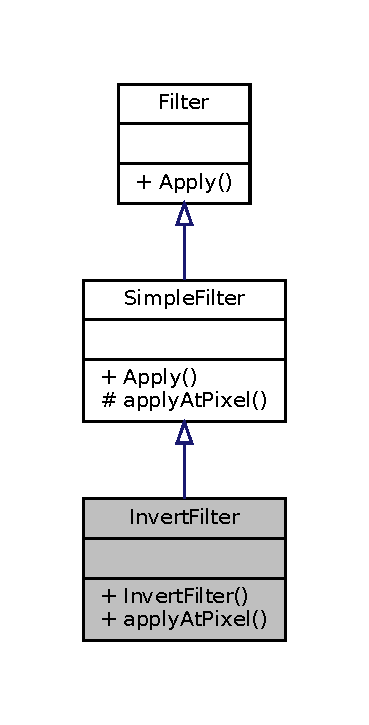
\includegraphics[width=177pt]{classInvertFilter__inherit__graph}
\end{center}
\end{figure}


Collaboration diagram for Invert\+Filter\+:
\nopagebreak
\begin{figure}[H]
\begin{center}
\leavevmode
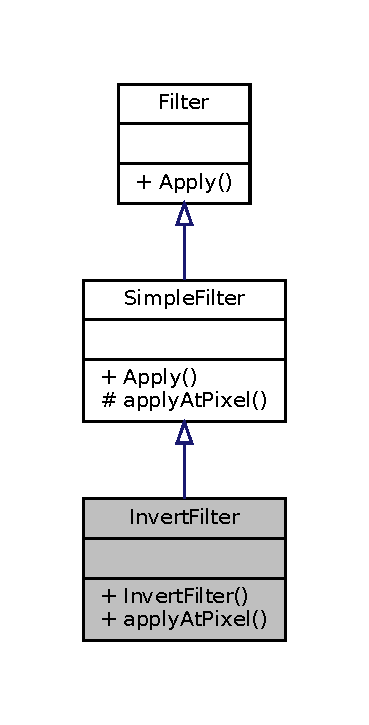
\includegraphics[width=177pt]{classInvertFilter__coll__graph}
\end{center}
\end{figure}
\subsection*{Public Member Functions}
\begin{DoxyCompactItemize}
\item 
\mbox{\Hypertarget{classInvertFilter_a30c32de66e0b4cd40174af651185d955}\label{classInvertFilter_a30c32de66e0b4cd40174af651185d955}} 
\hyperlink{classInvertFilter_a30c32de66e0b4cd40174af651185d955}{Invert\+Filter} ()
\begin{DoxyCompactList}\small\item\em Generation of an \hyperlink{classInvertFilter}{Invert\+Filter} with no parameters. \end{DoxyCompactList}\item 
\mbox{\Hypertarget{classInvertFilter_a440496aa9fb53511c32e451aaefb52a4}\label{classInvertFilter_a440496aa9fb53511c32e451aaefb52a4}} 
unsigned char $\ast$ \hyperlink{classInvertFilter_a440496aa9fb53511c32e451aaefb52a4}{apply\+At\+Pixel} (unsigned char $\ast$pixel)
\begin{DoxyCompactList}\small\item\em Application of an \hyperlink{classInvertFilter}{Invert\+Filter} at a specific pixel in the image. \end{DoxyCompactList}\end{DoxyCompactItemize}
\subsection*{Additional Inherited Members}


\subsection{Detailed Description}
The main class of \hyperlink{classInvertFilter}{Invert\+Filter}. 

Derived class of \hyperlink{classSimpleFilter}{Simple\+Filter}, invoked to create and apply an inversion filter to an \hyperlink{classImage}{Image}. 

The documentation for this class was generated from the following files\+:\begin{DoxyCompactItemize}
\item 
/home/user/repo/invert.\+h\item 
/home/user/repo/invert.\+cc\end{DoxyCompactItemize}

\hypertarget{classKernal}{}\doxysection{Kernal Class Reference}
\label{classKernal}\index{Kernal@{Kernal}}


a class for creating kernals to be used with convolutional filters;  




{\ttfamily \#include $<$kernal.\+h$>$}



Collaboration diagram for Kernal\+:\nopagebreak
\begin{figure}[H]
\begin{center}
\leavevmode
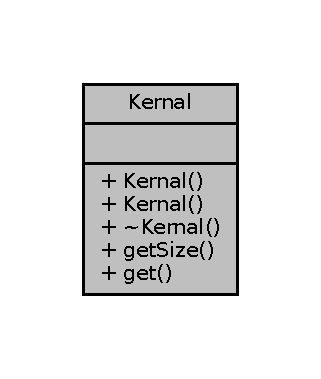
\includegraphics[width=154pt]{classKernal__coll__graph}
\end{center}
\end{figure}
\doxysubsection*{Public Member Functions}
\begin{DoxyCompactItemize}
\item 
\mbox{\hyperlink{classKernal_a6c583be3479e032ae54f74168098da5d}{Kernal}} (std\+::vector$<$ std\+::vector$<$ float $>$$>$ k)
\begin{DoxyCompactList}\small\item\em constructor for a \mbox{\hyperlink{classKernal}{Kernal}} that takes in a 2D vector; \end{DoxyCompactList}\item 
\mbox{\hyperlink{classKernal_a6b9b76d7863d4984485ed34cb492f12c}{Kernal}} ()
\begin{DoxyCompactList}\small\item\em default constructor for a \mbox{\hyperlink{classKernal}{Kernal}}; \end{DoxyCompactList}\item 
\mbox{\hyperlink{classKernal_aab6e0d2f014ad2f828bbbd8236cdeedc}{$\sim$\+Kernal}} ()
\begin{DoxyCompactList}\small\item\em destructor for a kernal; \end{DoxyCompactList}\item 
int \mbox{\hyperlink{classKernal_a0767772b0bf3f7eacb910fcd9ae1bfcc}{get\+Size}} ()
\begin{DoxyCompactList}\small\item\em getter for the size of a kernal; \end{DoxyCompactList}\item 
float \mbox{\hyperlink{classKernal_a4dfa813ba722fa66f40fb89443b23561}{get}} (int x, int y)
\begin{DoxyCompactList}\small\item\em a getter for the value located at \mbox{\hyperlink{classKernal}{Kernal}}\mbox{[}y\mbox{]}\mbox{[}x\mbox{]}; \end{DoxyCompactList}\end{DoxyCompactItemize}


\doxysubsection{Detailed Description}
a class for creating kernals to be used with convolutional filters; 



\doxysubsection{Constructor \& Destructor Documentation}
\mbox{\Hypertarget{classKernal_a6c583be3479e032ae54f74168098da5d}\label{classKernal_a6c583be3479e032ae54f74168098da5d}} 
\index{Kernal@{Kernal}!Kernal@{Kernal}}
\index{Kernal@{Kernal}!Kernal@{Kernal}}
\doxysubsubsection{\texorpdfstring{Kernal()}{Kernal()}\hspace{0.1cm}{\footnotesize\ttfamily [1/2]}}
{\footnotesize\ttfamily Kernal\+::\+Kernal (\begin{DoxyParamCaption}\item[{std\+::vector$<$ std\+::vector$<$ float $>$$>$}]{k }\end{DoxyParamCaption})}



constructor for a \mbox{\hyperlink{classKernal}{Kernal}} that takes in a 2D vector; 

\begin{DoxyReturn}{Returns}
a \mbox{\hyperlink{classKernal}{Kernal}} object with that 2D vector; 
\end{DoxyReturn}
\mbox{\Hypertarget{classKernal_a6b9b76d7863d4984485ed34cb492f12c}\label{classKernal_a6b9b76d7863d4984485ed34cb492f12c}} 
\index{Kernal@{Kernal}!Kernal@{Kernal}}
\index{Kernal@{Kernal}!Kernal@{Kernal}}
\doxysubsubsection{\texorpdfstring{Kernal()}{Kernal()}\hspace{0.1cm}{\footnotesize\ttfamily [2/2]}}
{\footnotesize\ttfamily Kernal\+::\+Kernal (\begin{DoxyParamCaption}{ }\end{DoxyParamCaption})}



default constructor for a \mbox{\hyperlink{classKernal}{Kernal}}; 

\begin{DoxyReturn}{Returns}
a \mbox{\hyperlink{classKernal}{Kernal}} with a size of 0; 
\end{DoxyReturn}
\mbox{\Hypertarget{classKernal_aab6e0d2f014ad2f828bbbd8236cdeedc}\label{classKernal_aab6e0d2f014ad2f828bbbd8236cdeedc}} 
\index{Kernal@{Kernal}!````~Kernal@{$\sim$Kernal}}
\index{````~Kernal@{$\sim$Kernal}!Kernal@{Kernal}}
\doxysubsubsection{\texorpdfstring{$\sim$Kernal()}{~Kernal()}}
{\footnotesize\ttfamily Kernal\+::$\sim$\+Kernal (\begin{DoxyParamCaption}{ }\end{DoxyParamCaption})}



destructor for a kernal; 

\begin{DoxyReturn}{Returns}
none; 
\end{DoxyReturn}


\doxysubsection{Member Function Documentation}
\mbox{\Hypertarget{classKernal_a4dfa813ba722fa66f40fb89443b23561}\label{classKernal_a4dfa813ba722fa66f40fb89443b23561}} 
\index{Kernal@{Kernal}!get@{get}}
\index{get@{get}!Kernal@{Kernal}}
\doxysubsubsection{\texorpdfstring{get()}{get()}}
{\footnotesize\ttfamily float Kernal\+::get (\begin{DoxyParamCaption}\item[{int}]{x,  }\item[{int}]{y }\end{DoxyParamCaption})}



a getter for the value located at \mbox{\hyperlink{classKernal}{Kernal}}\mbox{[}y\mbox{]}\mbox{[}x\mbox{]}; 

\begin{DoxyReturn}{Returns}
the value at (x,y) as a float; 
\end{DoxyReturn}
\mbox{\Hypertarget{classKernal_a0767772b0bf3f7eacb910fcd9ae1bfcc}\label{classKernal_a0767772b0bf3f7eacb910fcd9ae1bfcc}} 
\index{Kernal@{Kernal}!getSize@{getSize}}
\index{getSize@{getSize}!Kernal@{Kernal}}
\doxysubsubsection{\texorpdfstring{getSize()}{getSize()}}
{\footnotesize\ttfamily int Kernal\+::get\+Size (\begin{DoxyParamCaption}{ }\end{DoxyParamCaption})}



getter for the size of a kernal; 

\begin{DoxyReturn}{Returns}
the size represented as an int; 
\end{DoxyReturn}


The documentation for this class was generated from the following files\+:\begin{DoxyCompactItemize}
\item 
/home/ivers743/3081\+\_\+f21/repo-\/team-\/22/\mbox{\hyperlink{kernal_8h}{kernal.\+h}}\item 
/home/ivers743/3081\+\_\+f21/repo-\/team-\/22/kernal.\+cc\end{DoxyCompactItemize}

\hypertarget{classNonMaxSuppression}{}\section{Non\+Max\+Suppression Class Reference}
\label{classNonMaxSuppression}\index{Non\+Max\+Suppression@{Non\+Max\+Suppression}}


The \hyperlink{classNonMaxSuppression}{Non\+Max\+Suppression} class used to apply a non-\/max suppression filter given a photo\textquotesingle{}s intensity and direction each of which must be stored as images of the same size. Works best when used following a sobel filter.  




{\ttfamily \#include $<$non\+\_\+max\+\_\+suppression.\+h$>$}



Inheritance diagram for Non\+Max\+Suppression\+:
\nopagebreak
\begin{figure}[H]
\begin{center}
\leavevmode
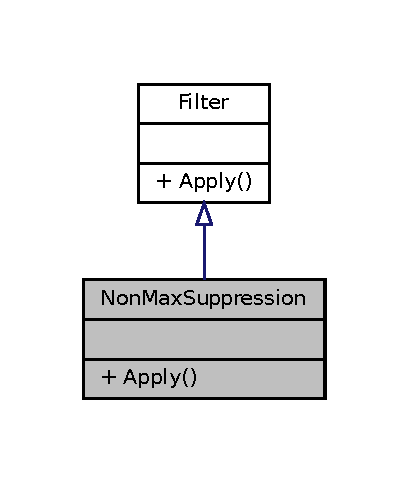
\includegraphics[width=196pt]{classNonMaxSuppression__inherit__graph}
\end{center}
\end{figure}


Collaboration diagram for Non\+Max\+Suppression\+:
\nopagebreak
\begin{figure}[H]
\begin{center}
\leavevmode
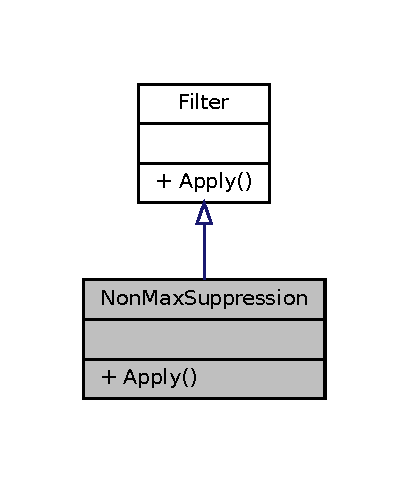
\includegraphics[width=196pt]{classNonMaxSuppression__coll__graph}
\end{center}
\end{figure}
\subsection*{Public Member Functions}
\begin{DoxyCompactItemize}
\item 
void \hyperlink{classNonMaxSuppression_a430a98e5683f8f70e7d8aaaa6efee5e8}{Apply} (std\+::vector$<$ \hyperlink{classImage}{Image} $\ast$$>$ input, std\+::vector$<$ \hyperlink{classImage}{Image} $\ast$$>$ output)
\begin{DoxyCompactList}\small\item\em Applies the filter. Intensity must be at index 0 and direction must be at index 1. Must be memory already allocated at the output. \end{DoxyCompactList}\end{DoxyCompactItemize}


\subsection{Detailed Description}
The \hyperlink{classNonMaxSuppression}{Non\+Max\+Suppression} class used to apply a non-\/max suppression filter given a photo\textquotesingle{}s intensity and direction each of which must be stored as images of the same size. Works best when used following a sobel filter. 

\subsection{Member Function Documentation}
\mbox{\Hypertarget{classNonMaxSuppression_a430a98e5683f8f70e7d8aaaa6efee5e8}\label{classNonMaxSuppression_a430a98e5683f8f70e7d8aaaa6efee5e8}} 
\index{Non\+Max\+Suppression@{Non\+Max\+Suppression}!Apply@{Apply}}
\index{Apply@{Apply}!Non\+Max\+Suppression@{Non\+Max\+Suppression}}
\subsubsection{\texorpdfstring{Apply()}{Apply()}}
{\footnotesize\ttfamily void Non\+Max\+Suppression\+::\+Apply (\begin{DoxyParamCaption}\item[{std\+::vector$<$ \hyperlink{classImage}{Image} $\ast$$>$}]{input,  }\item[{std\+::vector$<$ \hyperlink{classImage}{Image} $\ast$$>$}]{output }\end{DoxyParamCaption})\hspace{0.3cm}{\ttfamily [virtual]}}



Applies the filter. Intensity must be at index 0 and direction must be at index 1. Must be memory already allocated at the output. 

\begin{DoxyReturn}{Returns}
void. Places result in the output vector. 
\end{DoxyReturn}


Implements \hyperlink{classFilter_afab0d50af44a19a370ebe46c69b8ff4e}{Filter}.



The documentation for this class was generated from the following files\+:\begin{DoxyCompactItemize}
\item 
/home/user/repo/\hyperlink{non__max__suppression_8h}{non\+\_\+max\+\_\+suppression.\+h}\item 
/home/user/repo/non\+\_\+max\+\_\+suppression.\+cc\end{DoxyCompactItemize}

\hypertarget{classSimpleFilter}{}\doxysection{Simple\+Filter Class Reference}
\label{classSimpleFilter}\index{SimpleFilter@{SimpleFilter}}


a class for creating simple filters;  




{\ttfamily \#include $<$simple\+\_\+filter.\+h$>$}



Inheritance diagram for Simple\+Filter\+:\nopagebreak
\begin{figure}[H]
\begin{center}
\leavevmode
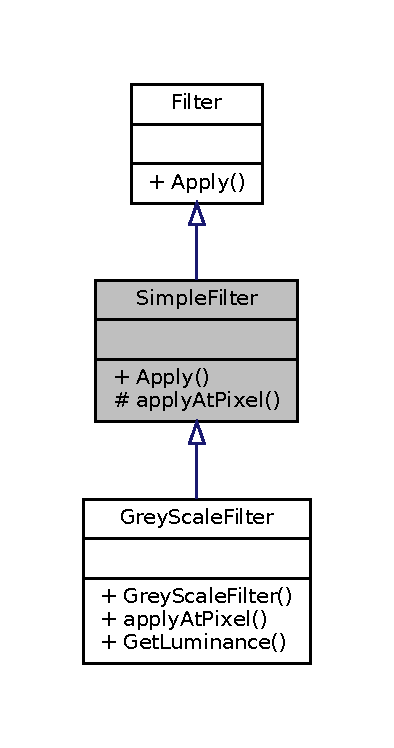
\includegraphics[width=350pt]{classSimpleFilter__inherit__graph}
\end{center}
\end{figure}


Collaboration diagram for Simple\+Filter\+:\nopagebreak
\begin{figure}[H]
\begin{center}
\leavevmode
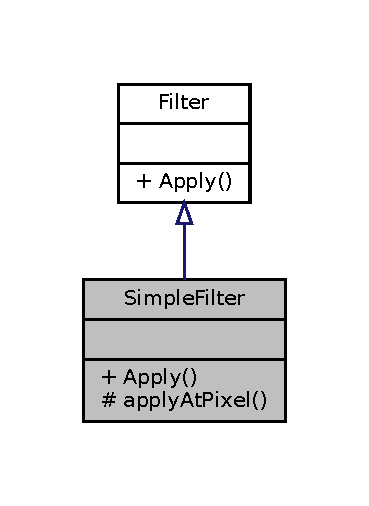
\includegraphics[width=177pt]{classSimpleFilter__coll__graph}
\end{center}
\end{figure}
\doxysubsection*{Public Member Functions}
\begin{DoxyCompactItemize}
\item 
void \mbox{\hyperlink{classSimpleFilter_a66dc06c85d8a38487e3dddc3e1731f37}{Apply}} (std\+::vector$<$ \mbox{\hyperlink{classImage}{Image}} $\ast$ $>$ original, std\+::vector$<$ \mbox{\hyperlink{classImage}{Image}} $\ast$ $>$ filtered)
\begin{DoxyCompactList}\small\item\em method to apply filter to an image, loops through image and calls apply\+At\+Pixel for every pixel; \end{DoxyCompactList}\end{DoxyCompactItemize}
\doxysubsection*{Protected Member Functions}
\begin{DoxyCompactItemize}
\item 
virtual unsigned char $\ast$ \mbox{\hyperlink{classSimpleFilter_a24100e6c29c4bf3bddf2763c22622d75}{apply\+At\+Pixel}} (unsigned char $\ast$pixel)=0
\begin{DoxyCompactList}\small\item\em virtual method, subclasses implement this method differently; \end{DoxyCompactList}\end{DoxyCompactItemize}


\doxysubsection{Detailed Description}
a class for creating simple filters; 



\doxysubsection{Member Function Documentation}
\mbox{\Hypertarget{classSimpleFilter_a66dc06c85d8a38487e3dddc3e1731f37}\label{classSimpleFilter_a66dc06c85d8a38487e3dddc3e1731f37}} 
\index{SimpleFilter@{SimpleFilter}!Apply@{Apply}}
\index{Apply@{Apply}!SimpleFilter@{SimpleFilter}}
\doxysubsubsection{\texorpdfstring{Apply()}{Apply()}}
{\footnotesize\ttfamily void Simple\+Filter\+::\+Apply (\begin{DoxyParamCaption}\item[{std\+::vector$<$ \mbox{\hyperlink{classImage}{Image}} $\ast$ $>$}]{original,  }\item[{std\+::vector$<$ \mbox{\hyperlink{classImage}{Image}} $\ast$ $>$}]{filtered }\end{DoxyParamCaption})\hspace{0.3cm}{\ttfamily [virtual]}}



method to apply filter to an image, loops through image and calls apply\+At\+Pixel for every pixel; 

\begin{DoxyReturn}{Returns}
nothing; 
\end{DoxyReturn}


Implements \mbox{\hyperlink{classFilter_a7431e1f16621d96f8a63b37b6907bb04}{Filter}}.

\mbox{\Hypertarget{classSimpleFilter_a24100e6c29c4bf3bddf2763c22622d75}\label{classSimpleFilter_a24100e6c29c4bf3bddf2763c22622d75}} 
\index{SimpleFilter@{SimpleFilter}!applyAtPixel@{applyAtPixel}}
\index{applyAtPixel@{applyAtPixel}!SimpleFilter@{SimpleFilter}}
\doxysubsubsection{\texorpdfstring{applyAtPixel()}{applyAtPixel()}}
{\footnotesize\ttfamily virtual unsigned char$\ast$ Simple\+Filter\+::apply\+At\+Pixel (\begin{DoxyParamCaption}\item[{unsigned char $\ast$}]{pixel }\end{DoxyParamCaption})\hspace{0.3cm}{\ttfamily [protected]}, {\ttfamily [pure virtual]}}



virtual method, subclasses implement this method differently; 

\begin{DoxyReturn}{Returns}
a length 4 character array; 
\end{DoxyReturn}


Implemented in \mbox{\hyperlink{classColorThresholdFilter_a6815edcf8ecf107e93006a5a610bacd0}{Color\+Threshold\+Filter}}, \mbox{\hyperlink{classDoubleThresholdFilter_ab6e5b2d489d32913b8cb1854d4ba6db2}{Double\+Threshold\+Filter}}, \mbox{\hyperlink{classGreyScaleFilter_afac3eb54599341d326d9df20de67f851}{Grey\+Scale\+Filter}}, and \mbox{\hyperlink{classInvertFilter_a440496aa9fb53511c32e451aaefb52a4}{Invert\+Filter}}.



The documentation for this class was generated from the following files\+:\begin{DoxyCompactItemize}
\item 
/home/ivers743/3081\+\_\+f21/repo-\/team-\/22/src/img\+\_\+proc\+\_\+src/simple\+\_\+filter.\+h\item 
/home/ivers743/3081\+\_\+f21/repo-\/team-\/22/src/img\+\_\+proc\+\_\+src/simple\+\_\+filter.\+cc\end{DoxyCompactItemize}

\hypertarget{classSobelFilter}{}\doxysection{Sobel\+Filter Class Reference}
\label{classSobelFilter}\index{SobelFilter@{SobelFilter}}


Sobel \mbox{\hyperlink{classFilter}{Filter}} class, allows for the creation of Sobel filters.  




{\ttfamily \#include $<$sobel\+\_\+filter.\+h$>$}



Inheritance diagram for Sobel\+Filter\+:\nopagebreak
\begin{figure}[H]
\begin{center}
\leavevmode
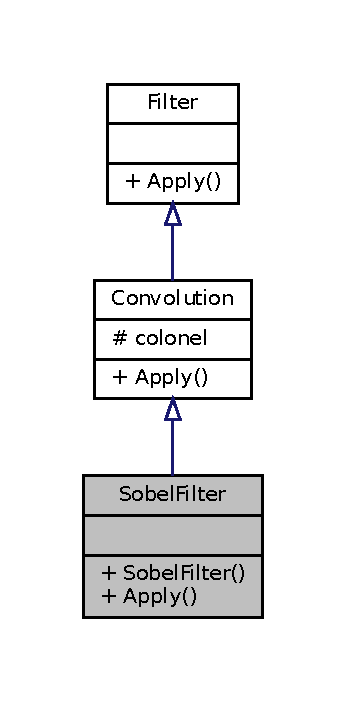
\includegraphics[width=166pt]{classSobelFilter__inherit__graph}
\end{center}
\end{figure}


Collaboration diagram for Sobel\+Filter\+:\nopagebreak
\begin{figure}[H]
\begin{center}
\leavevmode
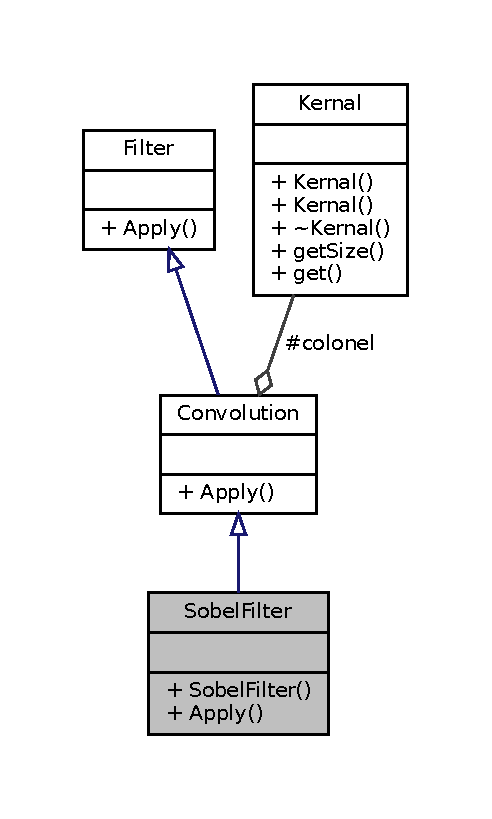
\includegraphics[width=236pt]{classSobelFilter__coll__graph}
\end{center}
\end{figure}
\doxysubsection*{Public Member Functions}
\begin{DoxyCompactItemize}
\item 
\mbox{\hyperlink{classSobelFilter_ae46218b3594451a1b5fbdf0ebbd7c688}{Sobel\+Filter}} ()
\begin{DoxyCompactList}\small\item\em constructor, sets colonel to the Sobel x identity matrix \end{DoxyCompactList}\item 
void \mbox{\hyperlink{classSobelFilter_a8cafdb5060028072077d4303840962ca}{Apply}} (std\+::vector$<$ \mbox{\hyperlink{classImage}{Image}} $\ast$ $>$ input, std\+::vector$<$ \mbox{\hyperlink{classImage}{Image}} $\ast$ $>$ output)
\begin{DoxyCompactList}\small\item\em method to apply a sobel filter to an image, note\+: takes in 2 output images \end{DoxyCompactList}\end{DoxyCompactItemize}
\doxysubsection*{Additional Inherited Members}


\doxysubsection{Detailed Description}
Sobel \mbox{\hyperlink{classFilter}{Filter}} class, allows for the creation of Sobel filters. 



\doxysubsection{Constructor \& Destructor Documentation}
\mbox{\Hypertarget{classSobelFilter_ae46218b3594451a1b5fbdf0ebbd7c688}\label{classSobelFilter_ae46218b3594451a1b5fbdf0ebbd7c688}} 
\index{SobelFilter@{SobelFilter}!SobelFilter@{SobelFilter}}
\index{SobelFilter@{SobelFilter}!SobelFilter@{SobelFilter}}
\doxysubsubsection{\texorpdfstring{SobelFilter()}{SobelFilter()}}
{\footnotesize\ttfamily Sobel\+Filter\+::\+Sobel\+Filter (\begin{DoxyParamCaption}{ }\end{DoxyParamCaption})}



constructor, sets colonel to the Sobel x identity matrix 



\doxysubsection{Member Function Documentation}
\mbox{\Hypertarget{classSobelFilter_a8cafdb5060028072077d4303840962ca}\label{classSobelFilter_a8cafdb5060028072077d4303840962ca}} 
\index{SobelFilter@{SobelFilter}!Apply@{Apply}}
\index{Apply@{Apply}!SobelFilter@{SobelFilter}}
\doxysubsubsection{\texorpdfstring{Apply()}{Apply()}}
{\footnotesize\ttfamily void Sobel\+Filter\+::\+Apply (\begin{DoxyParamCaption}\item[{std\+::vector$<$ \mbox{\hyperlink{classImage}{Image}} $\ast$ $>$}]{input,  }\item[{std\+::vector$<$ \mbox{\hyperlink{classImage}{Image}} $\ast$ $>$}]{output }\end{DoxyParamCaption})\hspace{0.3cm}{\ttfamily [virtual]}}



method to apply a sobel filter to an image, note\+: takes in 2 output images 



Implements \mbox{\hyperlink{classConvolution_aaeed86809bdfaa6b5723af9aa06f338c}{Convolution}}.



The documentation for this class was generated from the following files\+:\begin{DoxyCompactItemize}
\item 
/home/ivers743/3081\+\_\+f21/repo-\/team-\/22/src/img\+\_\+proc\+\_\+src/\mbox{\hyperlink{sobel__filter_8h}{sobel\+\_\+filter.\+h}}\item 
/home/ivers743/3081\+\_\+f21/repo-\/team-\/22/src/img\+\_\+proc\+\_\+src/sobel\+\_\+filter.\+cc\end{DoxyCompactItemize}

\hypertarget{structstbi__io__callbacks}{}\section{stbi\+\_\+io\+\_\+callbacks Struct Reference}
\label{structstbi__io__callbacks}\index{stbi\+\_\+io\+\_\+callbacks@{stbi\+\_\+io\+\_\+callbacks}}


Collaboration diagram for stbi\+\_\+io\+\_\+callbacks\+:
\nopagebreak
\begin{figure}[H]
\begin{center}
\leavevmode
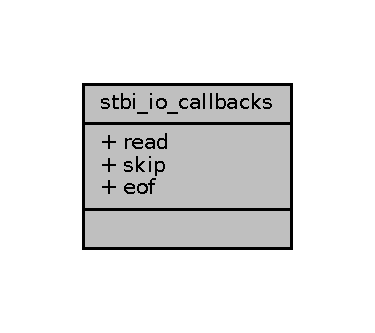
\includegraphics[width=180pt]{structstbi__io__callbacks__coll__graph}
\end{center}
\end{figure}
\subsection*{Public Attributes}
\begin{DoxyCompactItemize}
\item 
\mbox{\Hypertarget{structstbi__io__callbacks_a623e46b3a2a019611601409926283a88}\label{structstbi__io__callbacks_a623e46b3a2a019611601409926283a88}} 
int($\ast$ {\bfseries read} )(void $\ast$user, char $\ast$data, int size)
\item 
\mbox{\Hypertarget{structstbi__io__callbacks_a257aac5480a90a6c4b8fbe86c1b01068}\label{structstbi__io__callbacks_a257aac5480a90a6c4b8fbe86c1b01068}} 
void($\ast$ {\bfseries skip} )(void $\ast$user, int n)
\item 
\mbox{\Hypertarget{structstbi__io__callbacks_a319639db2f76e715eed7a7a974136832}\label{structstbi__io__callbacks_a319639db2f76e715eed7a7a974136832}} 
int($\ast$ {\bfseries eof} )(void $\ast$user)
\end{DoxyCompactItemize}


The documentation for this struct was generated from the following file\+:\begin{DoxyCompactItemize}
\item 
/home/user/repo/stb\+\_\+image.\+h\end{DoxyCompactItemize}

\chapter{File Documentation}
\hypertarget{convolution_8h}{}\doxysection{/home/ivers743/3081\+\_\+f21/repo-\/team-\/22/src/img\+\_\+proc\+\_\+src/convolution.h File Reference}
\label{convolution_8h}\index{/home/ivers743/3081\_f21/repo-\/team-\/22/src/img\_proc\_src/convolution.h@{/home/ivers743/3081\_f21/repo-\/team-\/22/src/img\_proc\_src/convolution.h}}
{\ttfamily \#include $<$vector$>$}\newline
{\ttfamily \#include \char`\"{}kernal.\+h\char`\"{}}\newline
{\ttfamily \#include \char`\"{}image.\+h\char`\"{}}\newline
{\ttfamily \#include \char`\"{}filter.\+h\char`\"{}}\newline
Include dependency graph for convolution.\+h\+:\nopagebreak
\begin{figure}[H]
\begin{center}
\leavevmode
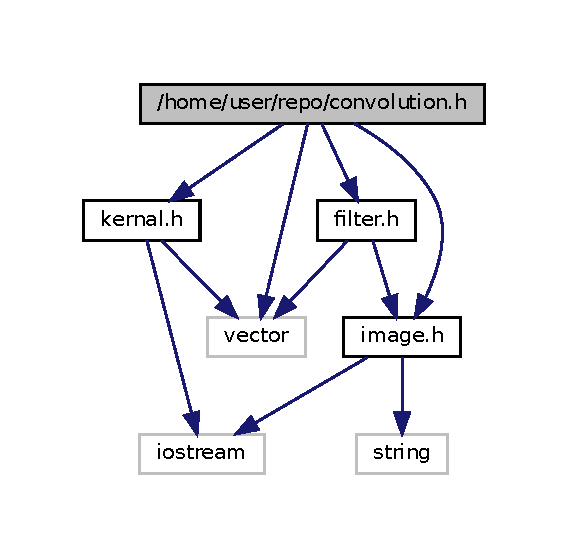
\includegraphics[width=280pt]{convolution_8h__incl}
\end{center}
\end{figure}
This graph shows which files directly or indirectly include this file\+:\nopagebreak
\begin{figure}[H]
\begin{center}
\leavevmode
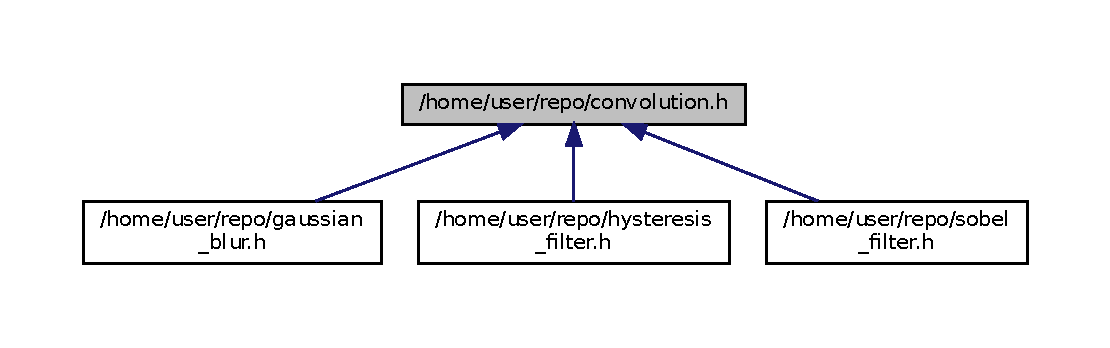
\includegraphics[width=350pt]{convolution_8h__dep__incl}
\end{center}
\end{figure}
\doxysubsection*{Classes}
\begin{DoxyCompactItemize}
\item 
class \mbox{\hyperlink{classConvolution}{Convolution}}
\begin{DoxyCompactList}\small\item\em The main class for convolutional filters, purely virtual. \end{DoxyCompactList}\end{DoxyCompactItemize}

\hypertarget{doublethreshold_8h}{}\section{/home/user/repo/doublethreshold.h File Reference}
\label{doublethreshold_8h}\index{/home/user/repo/doublethreshold.\+h@{/home/user/repo/doublethreshold.\+h}}
{\ttfamily \#include \char`\"{}simple\+\_\+filter.\+h\char`\"{}}\newline
Include dependency graph for doublethreshold.\+h\+:
\nopagebreak
\begin{figure}[H]
\begin{center}
\leavevmode
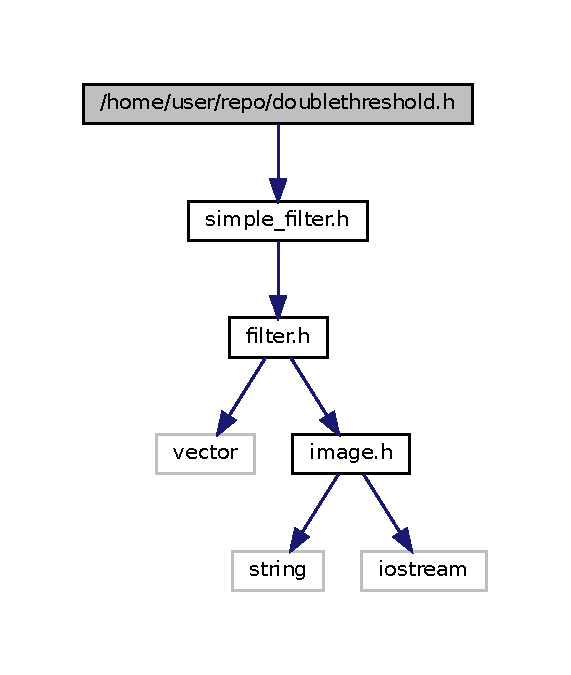
\includegraphics[width=274pt]{doublethreshold_8h__incl}
\end{center}
\end{figure}
\subsection*{Classes}
\begin{DoxyCompactItemize}
\item 
class \hyperlink{classDoubleThresholdFilter}{Double\+Threshold\+Filter}
\begin{DoxyCompactList}\small\item\em The main class of \hyperlink{classDoubleThresholdFilter}{Double\+Threshold\+Filter}. \end{DoxyCompactList}\end{DoxyCompactItemize}

\hypertarget{filter_8h}{}\doxysection{/home/ivers743/3081\+\_\+f21/repo-\/team-\/22/src/img\+\_\+proc\+\_\+src/filter.h File Reference}
\label{filter_8h}\index{/home/ivers743/3081\_f21/repo-\/team-\/22/src/img\_proc\_src/filter.h@{/home/ivers743/3081\_f21/repo-\/team-\/22/src/img\_proc\_src/filter.h}}
{\ttfamily \#include $<$vector$>$}\newline
{\ttfamily \#include \char`\"{}image.\+h\char`\"{}}\newline
Include dependency graph for filter.\+h\+:\nopagebreak
\begin{figure}[H]
\begin{center}
\leavevmode
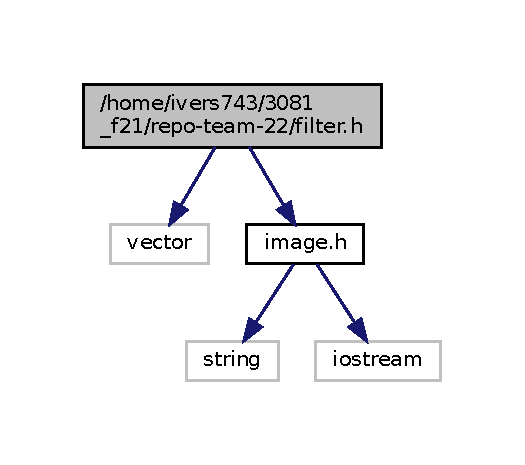
\includegraphics[width=275pt]{filter_8h__incl}
\end{center}
\end{figure}
This graph shows which files directly or indirectly include this file\+:\nopagebreak
\begin{figure}[H]
\begin{center}
\leavevmode
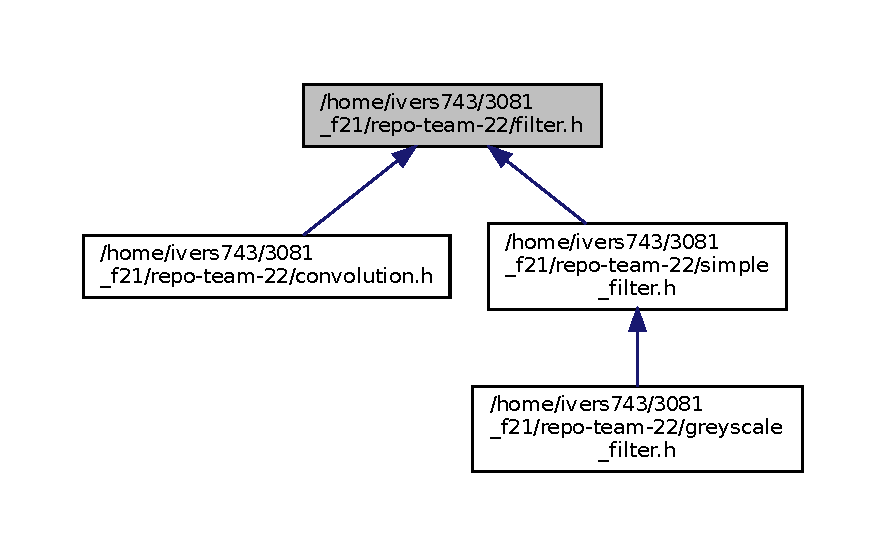
\includegraphics[width=350pt]{filter_8h__dep__incl}
\end{center}
\end{figure}
\doxysubsection*{Classes}
\begin{DoxyCompactItemize}
\item 
class \mbox{\hyperlink{classFilter}{Filter}}
\begin{DoxyCompactList}\small\item\em The main class for filters, purely virtual. \end{DoxyCompactList}\end{DoxyCompactItemize}

\hypertarget{gaussian__blur_8h}{}\section{/home/user/repo/gaussian\+\_\+blur.h File Reference}
\label{gaussian__blur_8h}\index{/home/user/repo/gaussian\+\_\+blur.\+h@{/home/user/repo/gaussian\+\_\+blur.\+h}}
{\ttfamily \#include \char`\"{}convolution.\+h\char`\"{}}\newline
{\ttfamily \#include $<$math.\+h$>$}\newline
Include dependency graph for gaussian\+\_\+blur.\+h\+:
\nopagebreak
\begin{figure}[H]
\begin{center}
\leavevmode
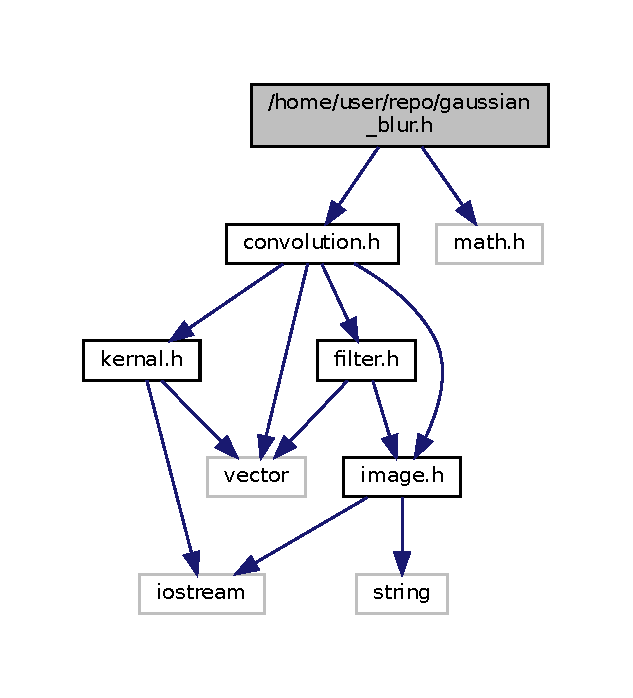
\includegraphics[width=304pt]{gaussian__blur_8h__incl}
\end{center}
\end{figure}
\subsection*{Classes}
\begin{DoxyCompactItemize}
\item 
class \hyperlink{classGaussian__Blur}{Gaussian\+\_\+\+Blur}
\begin{DoxyCompactList}\small\item\em Gaussian Blur class, allows for the creation of gaussian blur filters. \end{DoxyCompactList}\end{DoxyCompactItemize}

\hypertarget{greyscale__filter_8h}{}\doxysection{/home/ivers743/3081\+\_\+f21/repo-\/team-\/22/greyscale\+\_\+filter.h File Reference}
\label{greyscale__filter_8h}\index{/home/ivers743/3081\_f21/repo-\/team-\/22/greyscale\_filter.h@{/home/ivers743/3081\_f21/repo-\/team-\/22/greyscale\_filter.h}}
{\ttfamily \#include \char`\"{}simple\+\_\+filter.\+h\char`\"{}}\newline
Include dependency graph for greyscale\+\_\+filter.\+h\+:\nopagebreak
\begin{figure}[H]
\begin{center}
\leavevmode
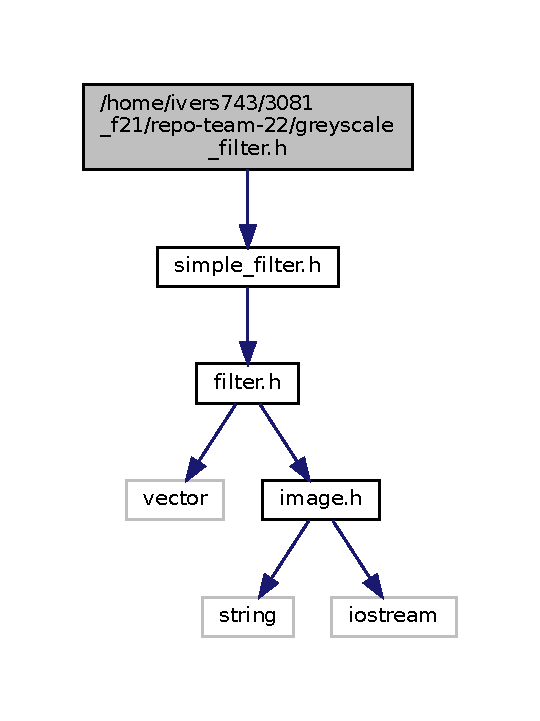
\includegraphics[width=259pt]{greyscale__filter_8h__incl}
\end{center}
\end{figure}
\doxysubsection*{Classes}
\begin{DoxyCompactItemize}
\item 
class \mbox{\hyperlink{classGreyScaleFilter}{Grey\+Scale\+Filter}}
\begin{DoxyCompactList}\small\item\em greyscale filter class, applies the greyscale filter to an image \end{DoxyCompactList}\end{DoxyCompactItemize}

\hypertarget{hysteresis__filter_8h}{}\section{/home/user/repo/hysteresis\+\_\+filter.h File Reference}
\label{hysteresis__filter_8h}\index{/home/user/repo/hysteresis\+\_\+filter.\+h@{/home/user/repo/hysteresis\+\_\+filter.\+h}}
{\ttfamily \#include \char`\"{}convolution.\+h\char`\"{}}\newline
{\ttfamily \#include $<$math.\+h$>$}\newline
Include dependency graph for hysteresis\+\_\+filter.\+h\+:
\nopagebreak
\begin{figure}[H]
\begin{center}
\leavevmode
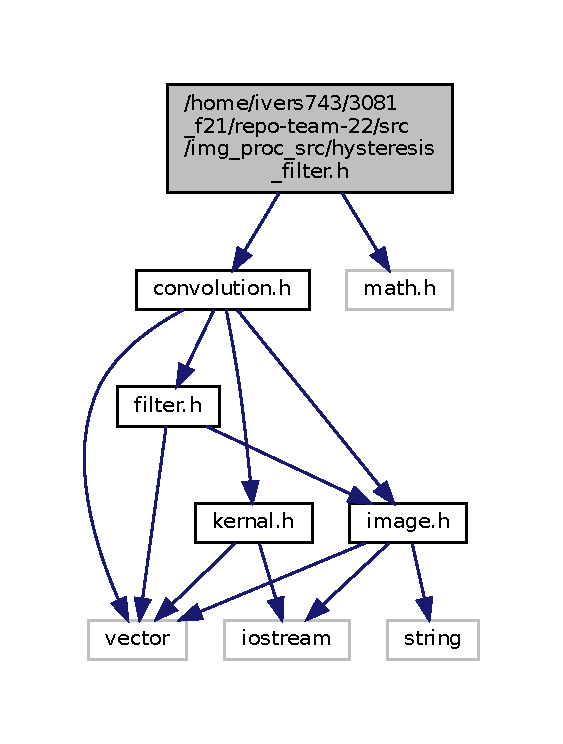
\includegraphics[width=307pt]{hysteresis__filter_8h__incl}
\end{center}
\end{figure}
\subsection*{Classes}
\begin{DoxyCompactItemize}
\item 
class \hyperlink{classHysteresisFilter}{Hysteresis\+Filter}
\begin{DoxyCompactList}\small\item\em Hysteresis \hyperlink{classFilter}{Filter} class, allows for the creation of hysteresis filters. \end{DoxyCompactList}\end{DoxyCompactItemize}

\hypertarget{image_8h}{}\doxysection{/home/ivers743/3081\+\_\+f21/repo-\/team-\/22/image.h File Reference}
\label{image_8h}\index{/home/ivers743/3081\_f21/repo-\/team-\/22/image.h@{/home/ivers743/3081\_f21/repo-\/team-\/22/image.h}}
{\ttfamily \#include $<$string$>$}\newline
{\ttfamily \#include $<$iostream$>$}\newline
Include dependency graph for image.\+h\+:\nopagebreak
\begin{figure}[H]
\begin{center}
\leavevmode
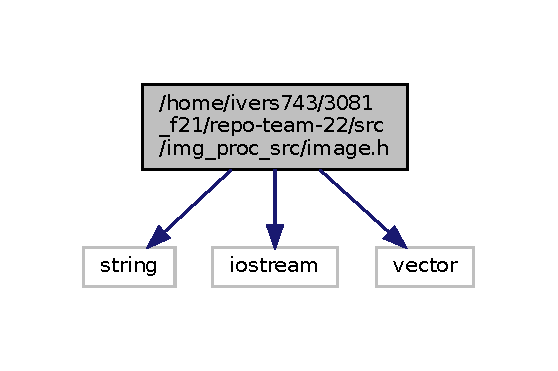
\includegraphics[width=230pt]{image_8h__incl}
\end{center}
\end{figure}
This graph shows which files directly or indirectly include this file\+:\nopagebreak
\begin{figure}[H]
\begin{center}
\leavevmode
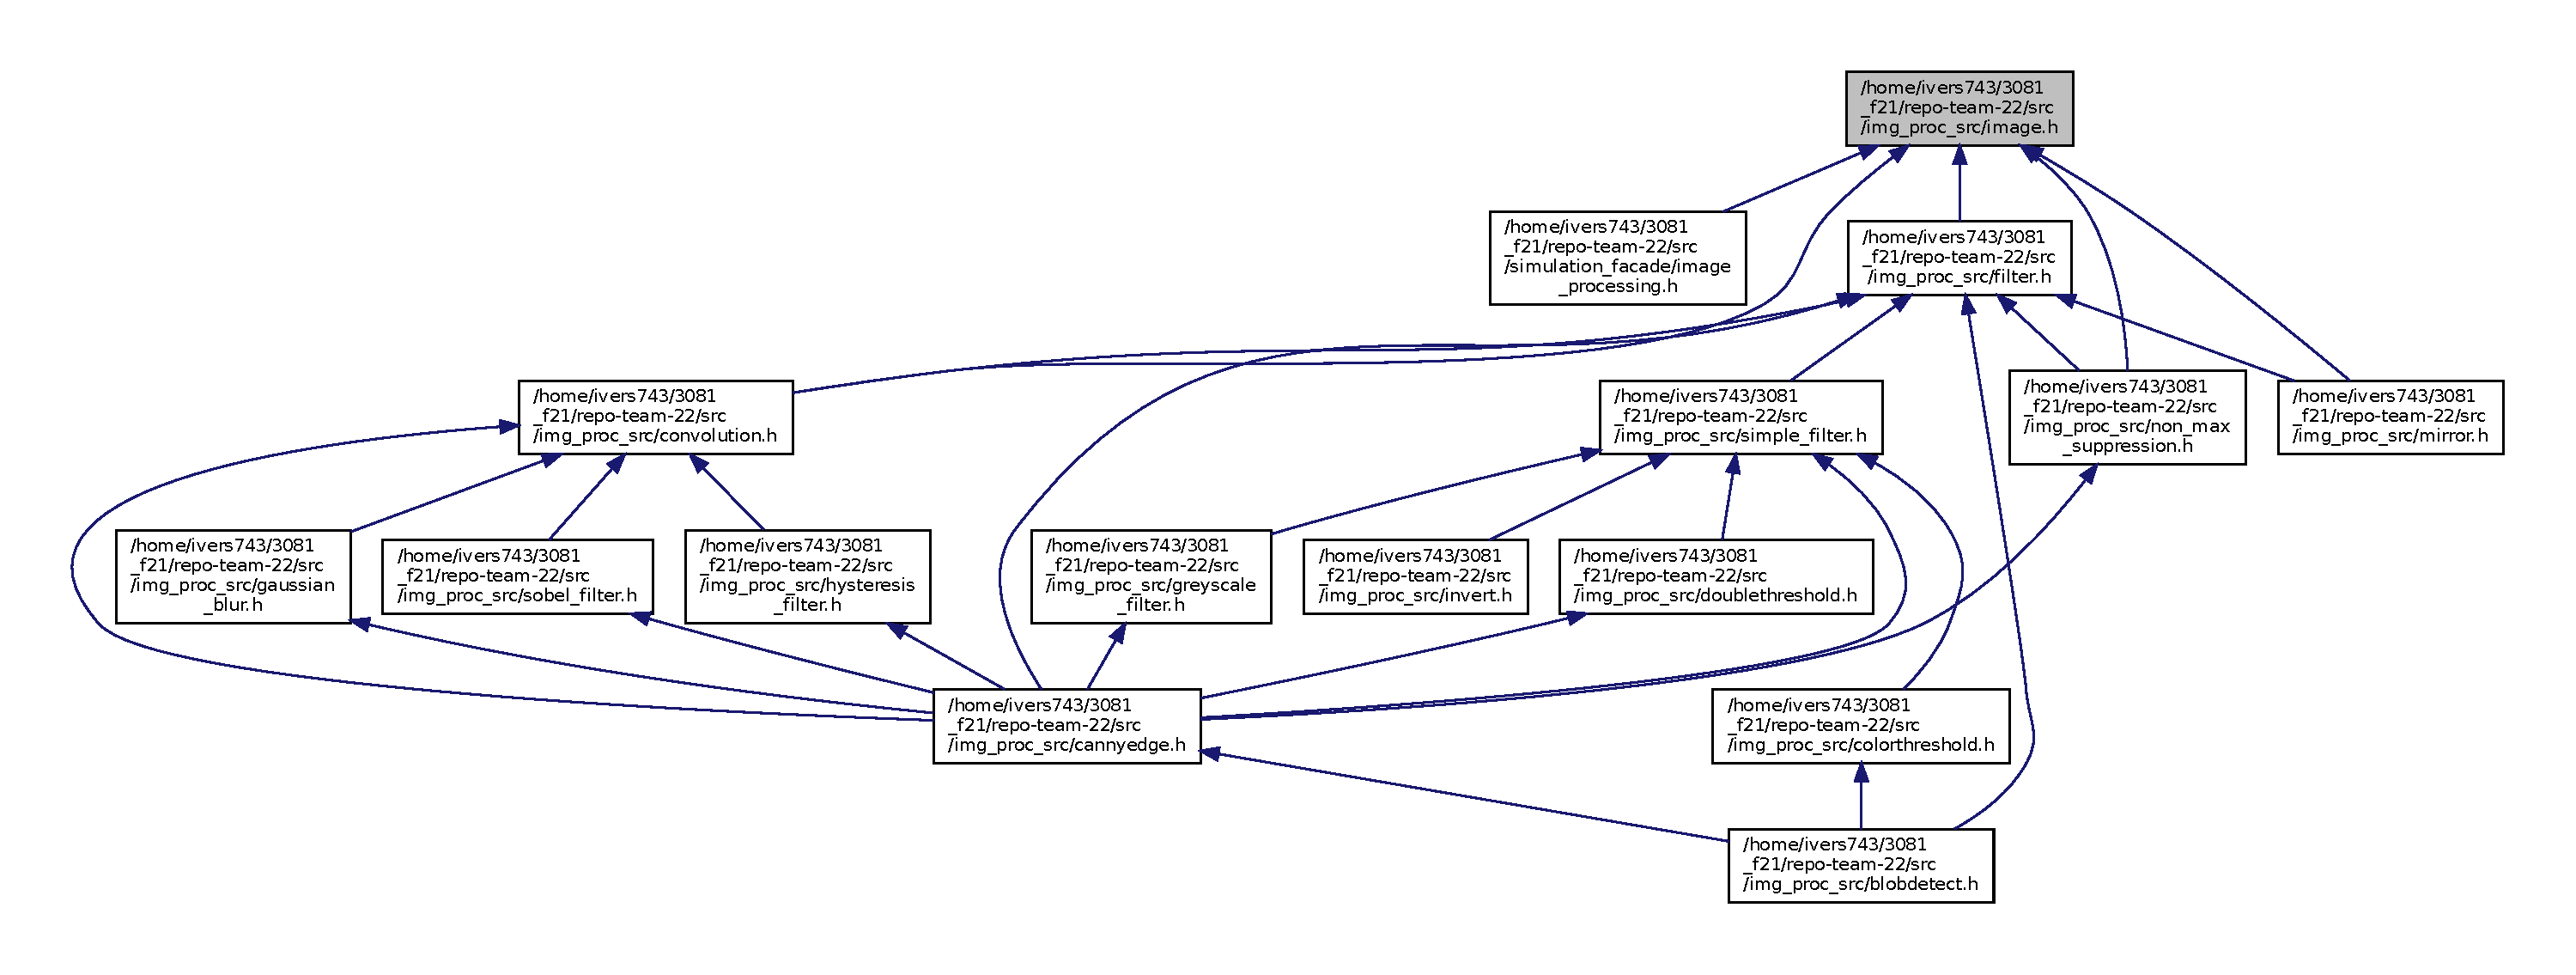
\includegraphics[width=350pt]{image_8h__dep__incl}
\end{center}
\end{figure}
\doxysubsection*{Classes}
\begin{DoxyCompactItemize}
\item 
class \mbox{\hyperlink{classImage}{Image}}
\begin{DoxyCompactList}\small\item\em The main class for images, allows for copying, saving, and getting/setting pixels. \end{DoxyCompactList}\end{DoxyCompactItemize}

\hypertarget{kernal_8h}{}\doxysection{/home/ivers743/3081\+\_\+f21/repo-\/team-\/22/kernal.h File Reference}
\label{kernal_8h}\index{/home/ivers743/3081\_f21/repo-\/team-\/22/kernal.h@{/home/ivers743/3081\_f21/repo-\/team-\/22/kernal.h}}
{\ttfamily \#include $<$vector$>$}\newline
{\ttfamily \#include $<$iostream$>$}\newline
Include dependency graph for kernal.\+h\+:\nopagebreak
\begin{figure}[H]
\begin{center}
\leavevmode
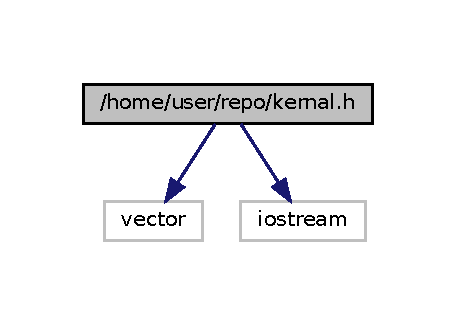
\includegraphics[width=229pt]{kernal_8h__incl}
\end{center}
\end{figure}
This graph shows which files directly or indirectly include this file\+:\nopagebreak
\begin{figure}[H]
\begin{center}
\leavevmode
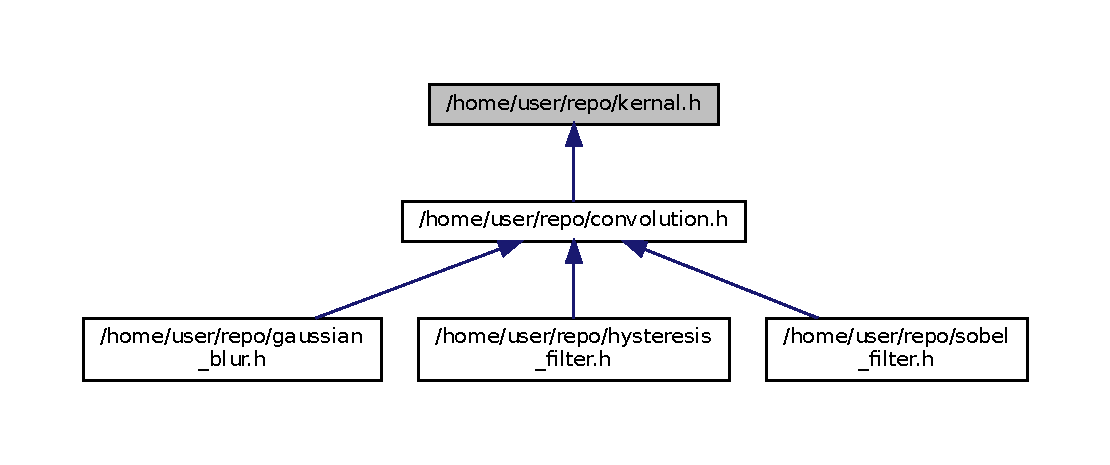
\includegraphics[width=256pt]{kernal_8h__dep__incl}
\end{center}
\end{figure}
\doxysubsection*{Classes}
\begin{DoxyCompactItemize}
\item 
class \mbox{\hyperlink{classKernal}{Kernal}}
\begin{DoxyCompactList}\small\item\em a class for creating kernals to be used with convolutional filters; \end{DoxyCompactList}\end{DoxyCompactItemize}

\hypertarget{non__max__suppression_8h}{}\section{/home/user/repo/non\+\_\+max\+\_\+suppression.h File Reference}
\label{non__max__suppression_8h}\index{/home/user/repo/non\+\_\+max\+\_\+suppression.\+h@{/home/user/repo/non\+\_\+max\+\_\+suppression.\+h}}
{\ttfamily \#include $<$vector$>$}\newline
{\ttfamily \#include \char`\"{}image.\+h\char`\"{}}\newline
{\ttfamily \#include \char`\"{}filter.\+h\char`\"{}}\newline
Include dependency graph for non\+\_\+max\+\_\+suppression.\+h\+:
\nopagebreak
\begin{figure}[H]
\begin{center}
\leavevmode
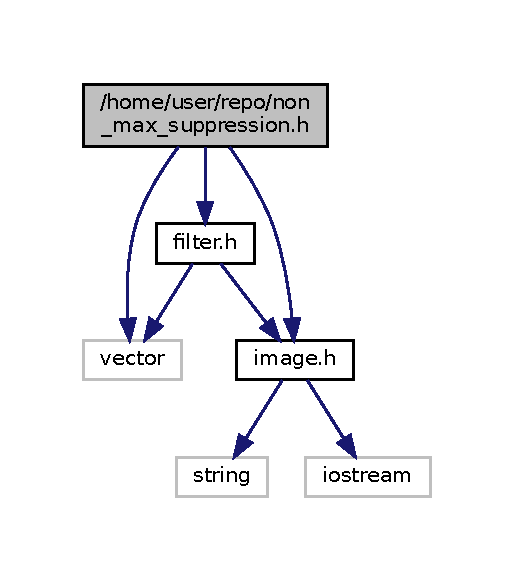
\includegraphics[width=247pt]{non__max__suppression_8h__incl}
\end{center}
\end{figure}
\subsection*{Classes}
\begin{DoxyCompactItemize}
\item 
class \hyperlink{classNonMaxSuppression}{Non\+Max\+Suppression}
\begin{DoxyCompactList}\small\item\em The \hyperlink{classNonMaxSuppression}{Non\+Max\+Suppression} class used to apply a non-\/max suppression filter given a photo\textquotesingle{}s intensity and direction each of which must be stored as images of the same size. Works best when used following a sobel filter. \end{DoxyCompactList}\end{DoxyCompactItemize}

\hypertarget{sobel__filter_8h}{}\doxysection{/home/ivers743/3081\+\_\+f21/repo-\/team-\/22/src/img\+\_\+proc\+\_\+src/sobel\+\_\+filter.h File Reference}
\label{sobel__filter_8h}\index{/home/ivers743/3081\_f21/repo-\/team-\/22/src/img\_proc\_src/sobel\_filter.h@{/home/ivers743/3081\_f21/repo-\/team-\/22/src/img\_proc\_src/sobel\_filter.h}}
{\ttfamily \#include \char`\"{}convolution.\+h\char`\"{}}\newline
{\ttfamily \#include $<$math.\+h$>$}\newline
Include dependency graph for sobel\+\_\+filter.\+h\+:\nopagebreak
\begin{figure}[H]
\begin{center}
\leavevmode
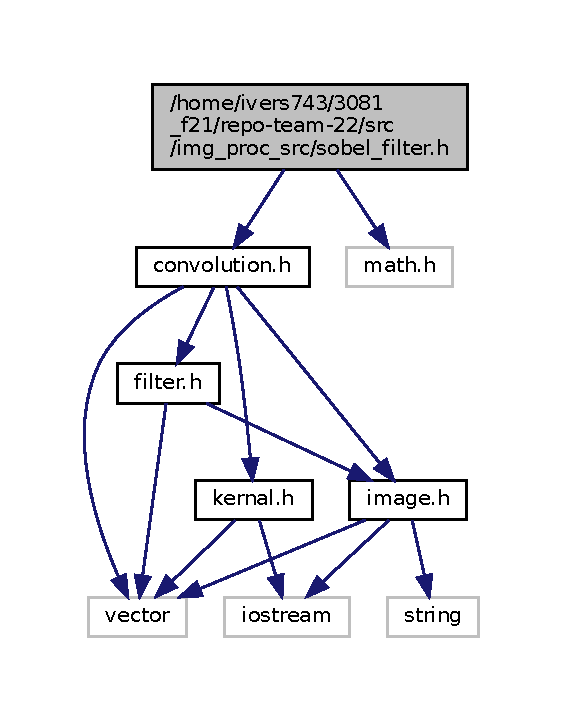
\includegraphics[width=270pt]{sobel__filter_8h__incl}
\end{center}
\end{figure}
This graph shows which files directly or indirectly include this file\+:\nopagebreak
\begin{figure}[H]
\begin{center}
\leavevmode
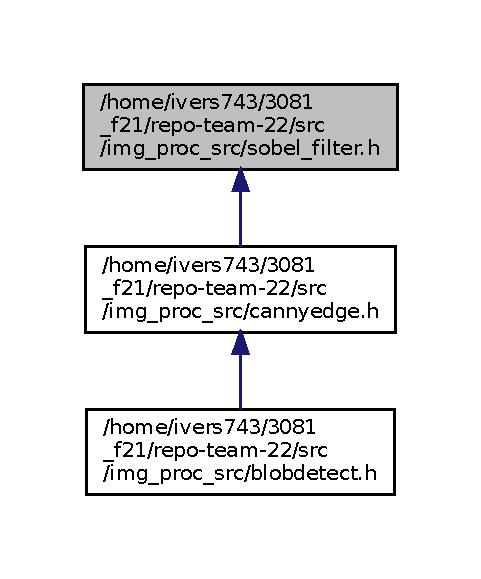
\includegraphics[width=231pt]{sobel__filter_8h__dep__incl}
\end{center}
\end{figure}
\doxysubsection*{Classes}
\begin{DoxyCompactItemize}
\item 
class \mbox{\hyperlink{classSobelFilter}{Sobel\+Filter}}
\begin{DoxyCompactList}\small\item\em Sobel \mbox{\hyperlink{classFilter}{Filter}} class, allows for the creation of Sobel filters. \end{DoxyCompactList}\end{DoxyCompactItemize}

%--- End generated contents ---

% Index
\backmatter
\newpage
\phantomsection
\clearemptydoublepage
\addcontentsline{toc}{chapter}{Index}
\printindex

\end{document}
